\Chapter{Étude de plasmas magnétisés}
\chaptermark{Étude de plasmas magnétisés}
\label{EtudePlasmaMag}
\begin{refsection}
Ce cinquième chapitre porte sur l'étude de trois cas de test simplifiés,
inspirés d'expérimentations réelles. Chacun des cas possède sa problématique
spécifique, et est représentatif d'une configuration magnétique
particulière :

\begin{itemize}
  \item le filtre magnétique avec le propulseur PEGASES
  \item la colonne de plasma magnétisée de la source d'ions négatifs CYBELE
  \item une région de bord de tokamak fortement magnétisée
\end{itemize}

À travers ces exemples très différents, nous testons les possibilités du nouveau
code MAGNIS, tout en explorant la physique qu'il révèle. Les simulations sont discutées et
les phénomènes observés confrontés aux observations expérimentales et
numériques.

\section{Barrière magnétique - PEGASES}
\subsection{La géométrie barrière magnétique}
Le champ magnétique en configuration de filtre (ou de barrière)
est un élément essentiel au fonctionnement de certaines sources d'ions
négatifs. Le principe de ces sources, comme rappelé dans la
figure~\ref{IPPIonSource2}, est de constituer une région de faible température
électronique (condition nécessaire à la création
et la survie des ions négatifs) en appliquant localement un champ magnétique
dans la direction transverse. Cette configuration est reconnue pour avoir un
comportement complexe, et mener à différentes asymétries dans le plasma,
notamment sur le flux électronique, comme montré sur la
figure~\ref{IPPIonSourcecourant2}.

\vspace{5 mm}
\begin{minipage}{0.9\textwidth}
\begin{minipage}{0.5\textwidth}
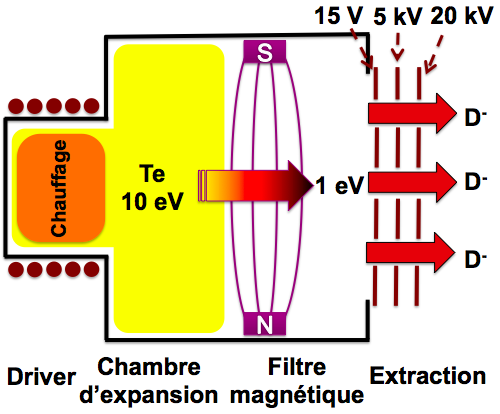
\includegraphics[width=1\textwidth]{figures/sourceIPP.png}
\captionsetup{justification=raggedright, singlelinecheck=false}
\captionof{figure}{Schéma de principe de l'un des "driver" de la source d'ions
négatifs de l'IPP Garching.}\label{IPPIonSource2}
\end{minipage}\qquad\qquad
\begin{minipage}{0.40\textwidth}
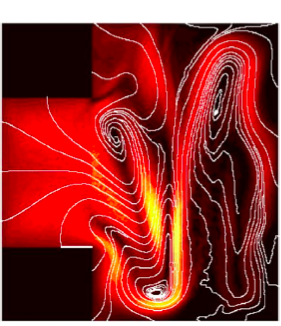
\includegraphics[width=0.9\textwidth]{figures/sourceIPPcourant.png}
\captionsetup{justification=raggedright, singlelinecheck=false}
\captionof{figure}{Dérive du flux électronique
le long de la barrière de champ magnétique.}\label{IPPIonSourcecourant2}
\end{minipage}
\end{minipage}
\vspace{5 mm}

Pour valider le modèle de MAGNIS, le cas de test de la barrière magnétique est
incontournable. Entre la source d'ions négatifs d'ITER, qui a déjà fait l'objet
de quantités de publications, la manipulation expérimentale de METRIS, dont la
configuration générale et la géométrie exacte est assez complexe et le propulseur PEGASES,
nous choisissons de présenter ce dernier pour plusieurs raisons : 

\begin{itemize}
  \item PEGASES a tout d'abord une géométrie rectangulaire bien adaptée à notre
  modèle 
  \item il y a ensuite de nombreuses données expérimentales disponibles pour
  effectuer des comparaisons quantitatives
  \item PEGASES opère entre autres avec un gaz d'argon, ce
  qui est très intéressant pour tester la prise en compte de l'inertie dans le
  modèle
  \item enfin, certains des membres du GREPHE sont impliqués dans le projet ANR
  Blanc EPIC (LPP Polytechnique 2011) sur le propulseur et commencent à obtenir
  des résultats avec des modèles PIC dans ce contexte
\end{itemize}


\subsection{Le propulseur PEGASES}
PEGASES, acronyme de \emph{Plasma Propulsion with Electronegative GASES}, est
un prototype de propulseur électrostatique à grille (PEG)
ion-ion~\parencite{Chabert} conçu au LPP (Laboratoire de Physique des
Plasma) de l'École Polytechnique de Palaiseau, et dont l'originalité est
d'éjecter alternativement des ions négatifs et des ions positifs issus d'un plasma ion-ion continu.
Dans ce nouveau concept, les faisceaux d'ions de charges opposées se
neutralisent mutuellement à la sortie du propulseur, ce qui permet de se
libérer de l'utilisation de la cathode neutralisante habituellement requise
pour éviter la polarisation du dispositif.
Pour filtrer les électrons chauds et favoriser la création du plasma ion-ion, une
barrière magnétique d'une centaine de Gauss est placée entre la zone
d'ionisation et la région d'extraction. La structure en différents étages de PEGASES est représentée sur la
figure \ref{4-pegases3D} :

\begin{figure}[!htbp]
\centering
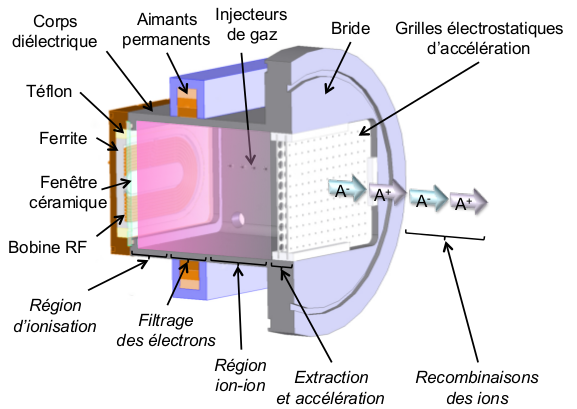
\includegraphics[width=0.75\textwidth]{figures/4-pegases3D.png}
{\caption{Schéma de principe de fonctionnement du propulseur PEGASES avec les
différents étages mentionnés en italiques\parencite{Popelier}.}
\label{4-pegases3D}}
\end{figure}

Dans le premier étage, un gaz électronégatif est
excité inductivement par une puissance RF.
Le plasma de la source, constitué d'ion positifs, d'ions négatifs et d'électrons
est ensuite filtré par une barrière magnétique dans le deuxième étage du
propulseur. L'intensité de la barrière magnétique est choisie de façon à ce que
seuls les électrons soient magnétisés, laissant les ions diffuser librement à
travers le champ. Le plasma se sépare ainsi en deux régions de températures
électroniques différentes, l'une chaude du côté de l'injection de puissance,
l'autre plus froide en aval de la barrière, où se forme un plasma
ion-ion. Le troisième étage est enfin constitué du plasma ion-ion et
d'une série de grilles que l'on polarise pour extraire et accélérer les
particules, afin de former les faisceaux d'ions qui feront la poussée. 

La source ICP est entretenue à 4~MHz avec une bobine plane dopée par un noyau de
ferrite protégée d'une fine (3~mm) couche de céramique\parencite{Godyak} qui
peut fournir une puissance allant de 50~W à 250~W\footnote{Dans le modèle, 
le chauffage n'est pas calculé mais modélisé par une puissance
absorbée totale, répartie en fonction de la zone de chauffage et de la densité
électronique.}. La géométrie de la source et la configuration du filtre magnétique ont été choisies d'après les résultats de Aanesland \emph{et al.}\parencite{Aanesland} qui donnent les conditions nécessaires à la
formation d'un plasma ion-ion. L'enceinte du propulseur, de dimension
12x12x8~cm$^3$, est usiné à partir d'un bloc d'aluminium, anodisé afin de rendre
ses parois diélectriques. Une autre version, constituée de parois conductrices,
est aussi utilisée à des fins de diagnostic pour les éléments de la source.

Pour étudier ce comportement, nous choisissons de
simuler un plasma d'argon, avec la géométrie présentée figure
\ref{4-pegasesSimDomain} :

\begin{figure}[!htbp]
\centering
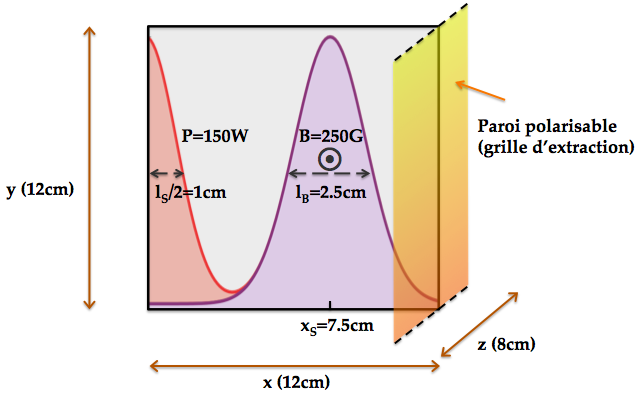
\includegraphics[width=0.7\textwidth]{figures/4-pegasesSimDomain.png}
{\caption{Le domaine de simulation est le plan perpendiculaire au champ
magnétique.}
\label{4-pegasesSimDomain}}
\end{figure}

\subsection{Simulation de base - Parois isolantes}

Le domaine de simulation est rectangulaire et de
dimensions similaires à celles du prototype. La puissance est déposée dans la
région en amont du filtre magnétique sous la forme d'une demi-gaussienne de 2 cm
de largeur. Le filtre magnétique est aussi de forme gaussienne, centré en
$x_\mathcal{S}\,$= 7.5 cm et de largeur $l_\mathcal{S}\sim\,$2.5 cm. Les parois
seront choisies conductrices ou diélectriques, avec une polarisation éventuelle de la grille
d'extraction (en jaune à droite du domaine). La puissance totale absorbée et la
densité de gaz sont fixées respectivement à 250~W et 1~mTorr. Ces paramètres
sont résumés dans le tableau~\ref{4-PegasesBaseParam}.

\begin{minipage}{\textwidth}
\footnotesize\centering
\ra{1.3}
\begin{tabular}{lcclc}\toprule
\multicolumn{5}{c}{\bf Paramètres}\\
\midrule 
Parois & Isolantes &&$L_x$, $L_y$, $L_z$  & 12cm, 12cm,
8cm\\
$\mathcal{P}_\text{ext}$&250W&&$l_\mathcal{S}$, $x_\mathcal{S}$&2cm, 0cm\\
$B$&250G&&$l_B$, $x_B$&2.5cm, 7.5cm\\
gaz (Ar) & 1 mTorr &&$\Delta t$, $\Delta x$&10$^{-8}$s,
1mm\\
\bottomrule
\end{tabular}
\captionof{table}{Paramètres de la simulation.}\label{4-PegasesBaseParam}
\end{minipage}

Les types de solutions obtenues par MAGNIS dans le cas de parois diélectriques
et sans bias appliqué sont illustrées sur les figures de \ref{4-CartesWithTe} :

\begin{figure}[!htbp]
    \centering
    \subfigure[]{\label{4-PegasesCarteDensiteBase}
    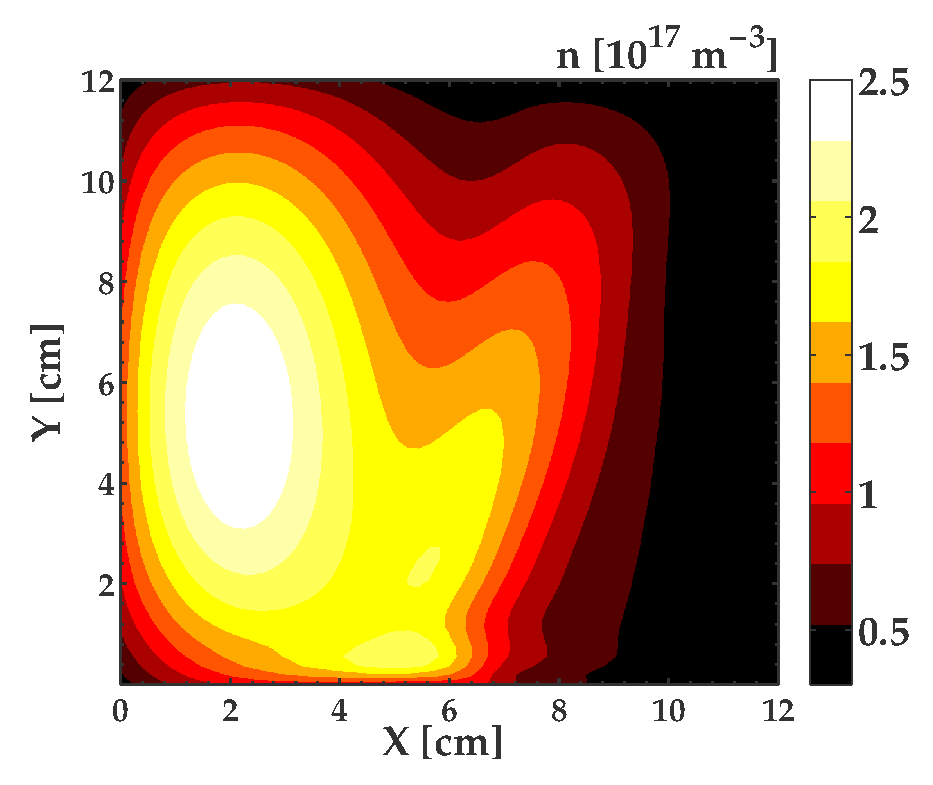
\includegraphics[height=5.75cm]{figures/4-PegasesCarteDensiteBase.eps}}
    \subfigure[]{\label{4-PegasesCartePotentielBase}
    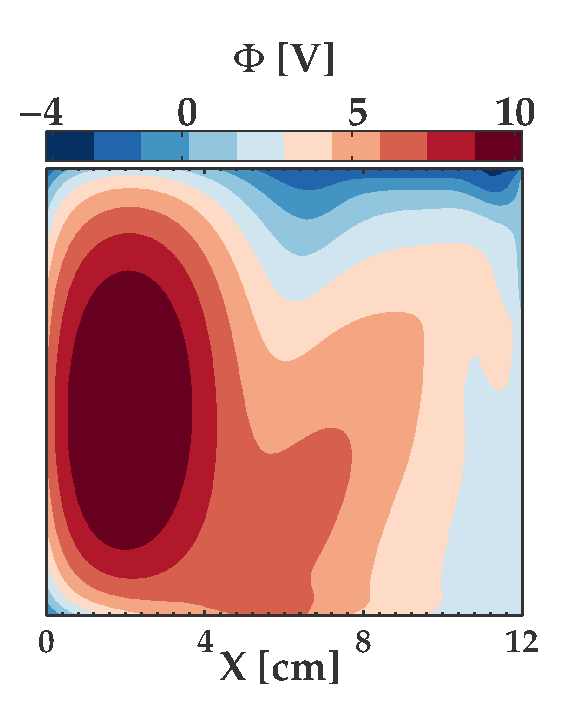
\includegraphics[height=5.75cm]{figures/4-PegasesCartePotentielBase.eps}}
    \subfigure[]{\label{4-PegasesCarteTemperatureBase}
    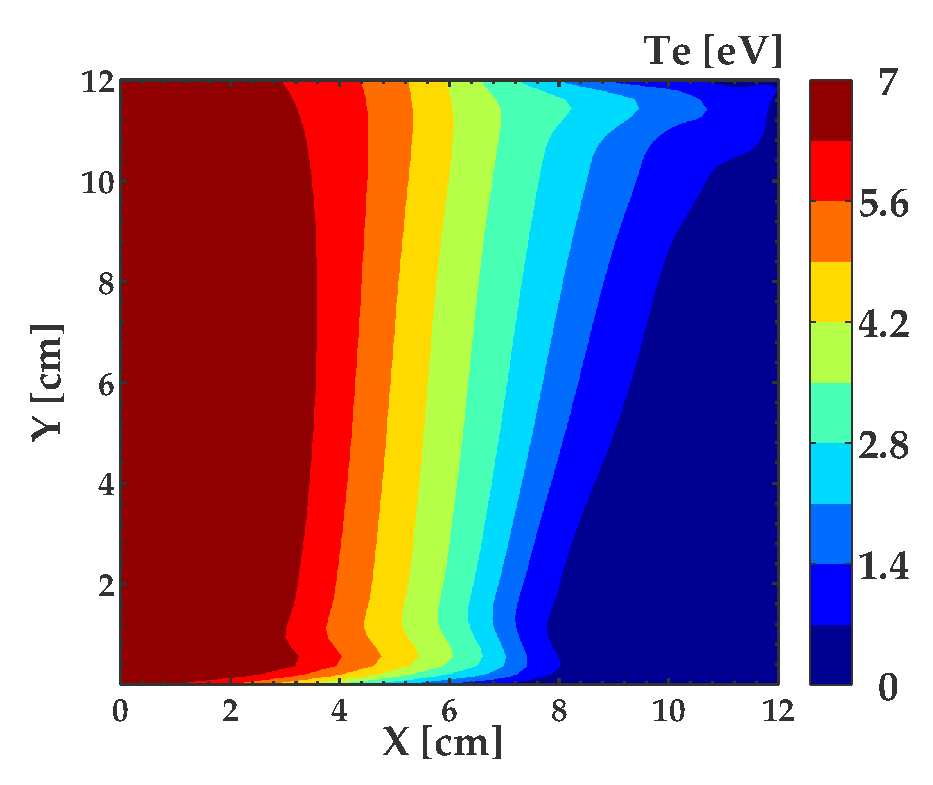
\includegraphics[height=5.75cm]{figures/4-PegasesCarteTemperatureBase.eps}}
    \caption{Cartes de densité \subref{4-PegasesCarteDensiteBase}~, de potentiel
    \subref{4-PegasesCartePotentielBase}~ et de température
    \subref{4-PegasesCarteTemperatureBase}~ dans le cas de parois
    diélectriques.}
    \label{4-CartesWithTe}
	\end{figure}

À partir de conditions initiales uniformes ($n_e\,$= 10$^{17}$ cm$^{-3}$ et
$T_e\,$= 5 eV), le plasma atteint un état stationnaire en $t\simeq\,$
10$^{-4}\,$s.
Le maximum de densité de la source, 2.5x10$^{17}\,$m$^{-3}$ est situé au
centre de la région d'ionisation. La densité du plasma décroît ensuite très
rapidement sur une longueur de 2 à 4 cm. 

Sur la figure~\ref{4-PegasesCarteDensiteBase} on reconnaît bien l'asymétrie
caractéristique du filtre magnétique qui se forme par rapport à l'axe
$y\,$=~6~cm : le plasma s'étend jusque dans la région du
filtre de façon non-uniforme.
La figure~\ref{4-PegasesCartePotentielBase} montre le potentiel
électrique $\Phi$. Il suit le profil de densité, et donne naissance à un champ
électrique d'une centaine de volt par mètre, quasiment ambipolaire dans la
région non magnétisée, et plutôt faible dans le filtre magnétique.

La carte de la température électronique $T_e$ est présentée sur la
figure~\ref{4-PegasesCarteTemperatureBase}. Le filtre magnétique fait fortement
décroître la température électronique, la faisant chuter de 7~eV à 1~eV sur une
longueur de quelques centimètres : dans le filtre, les électrons sont piégés le
long des lignes de champ, et refroidissent dans les collisions avec les neutres
qui continuent à leur enlever de l'énergie. Le transport thermique dans la
direction $x$ est alors considérablement diminué.
On peut aussi remarquer la légère asymétrie qui apparaît le long de la
direction $y$.

\begin{figure}[!htbp]\centering
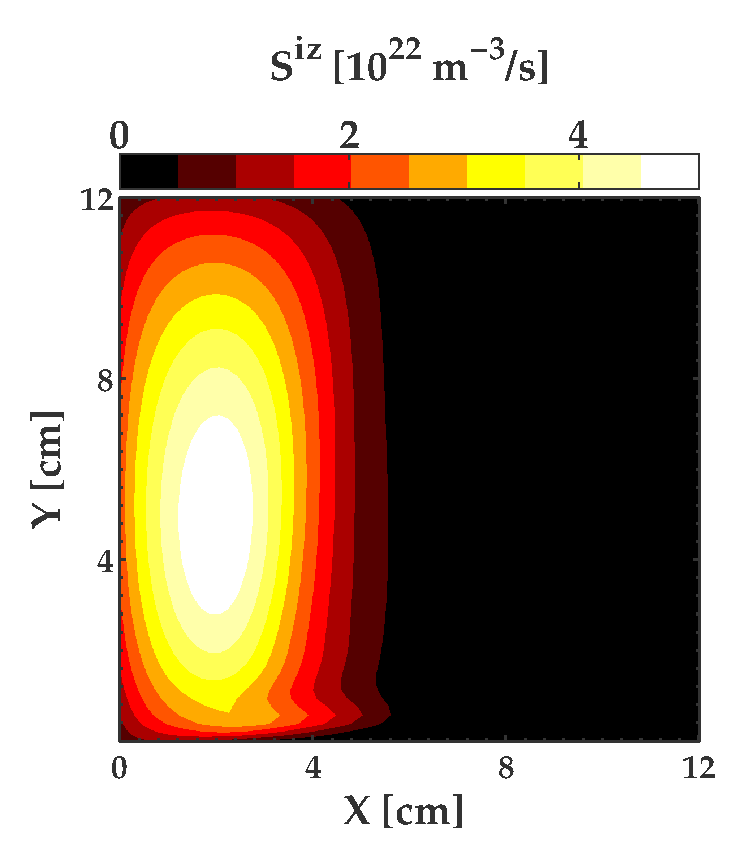
\includegraphics[height=6.5cm]{figures/4-PegasesCarteSourceBase.eps}
\caption{Source de particules provenant de l'ionisation.}
\label{4-PegasesCarteSourceBase}
\end{figure}

Dans les plasmas, le profil de densité s'établit en fonction de l'ionisation
et du transport. La figure~\ref{4-PegasesCarteSourceBase}, qui illustre le
nombre de particules ionisées par unité de temps et de volume, montre que dans ces
conditions le plasma est principalement créé en amont du champ magnétique.
C'est donc l'anisotropie du transport qui induit l'asymétrie. 

Dans ce type de configuration
magnétique les électrons, dont la mobilité est considérablement réduite en
travers du champ magnétique, cherchent un moyen de franchir le filtre afin de
retrouver les ions et préserver la quasineutralité du plasma. Les cartes de flux
ioniques et électroniques présentées sur la figure~\ref{4-PegasesCarteFlux}
permettent de se faire une idée de la dynamique du système. 

\begin{figure}[!htbp]
  \centering
    \subfigure[]{\label{4-PegasesCarteFluxIBase}
    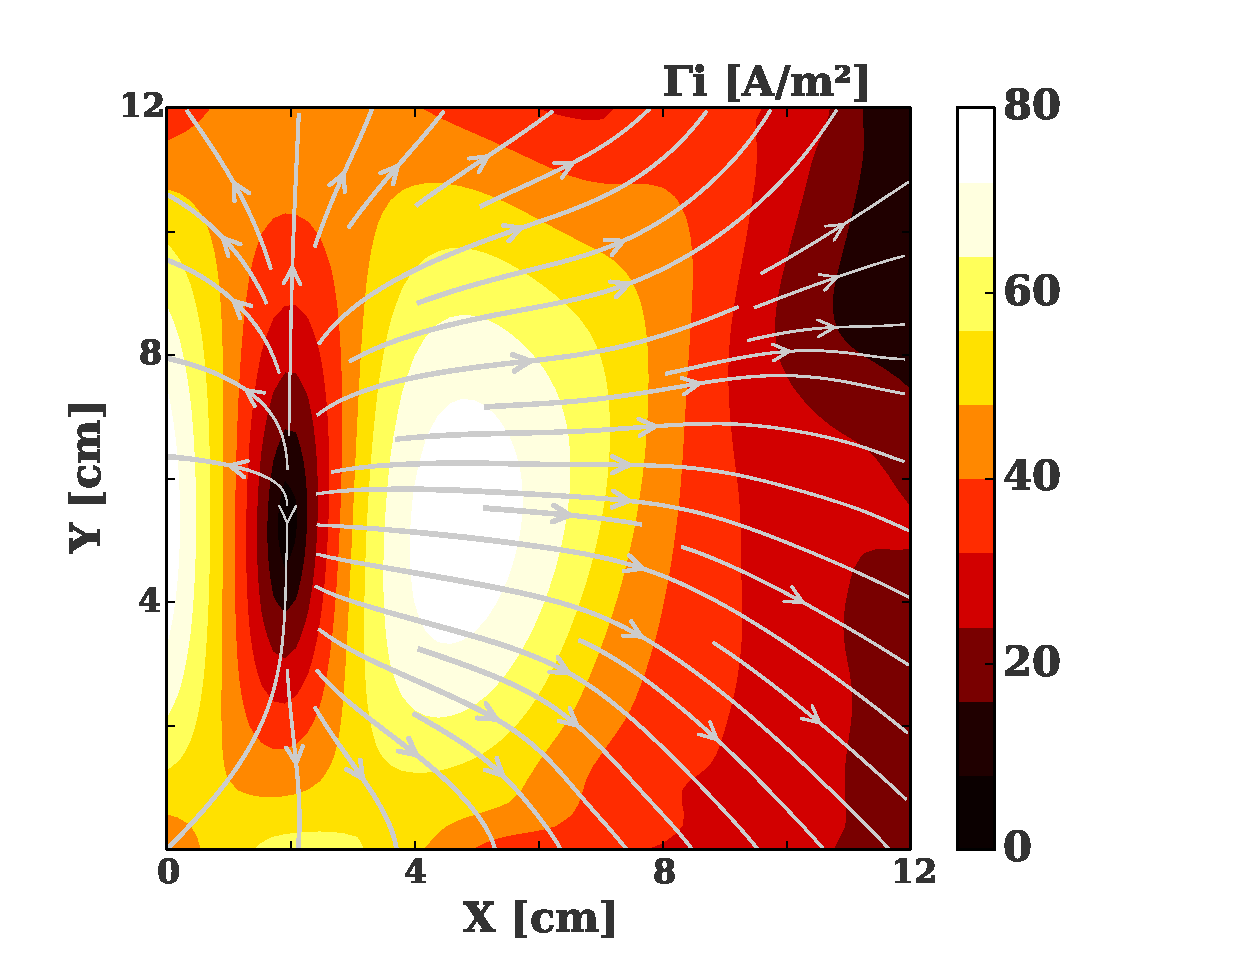
\includegraphics[height=6cm]{figures/4-PegasesCarteFluxIBase.eps}}
    \subfigure[]{\label{4-PegasesCarteFluxEBase}
    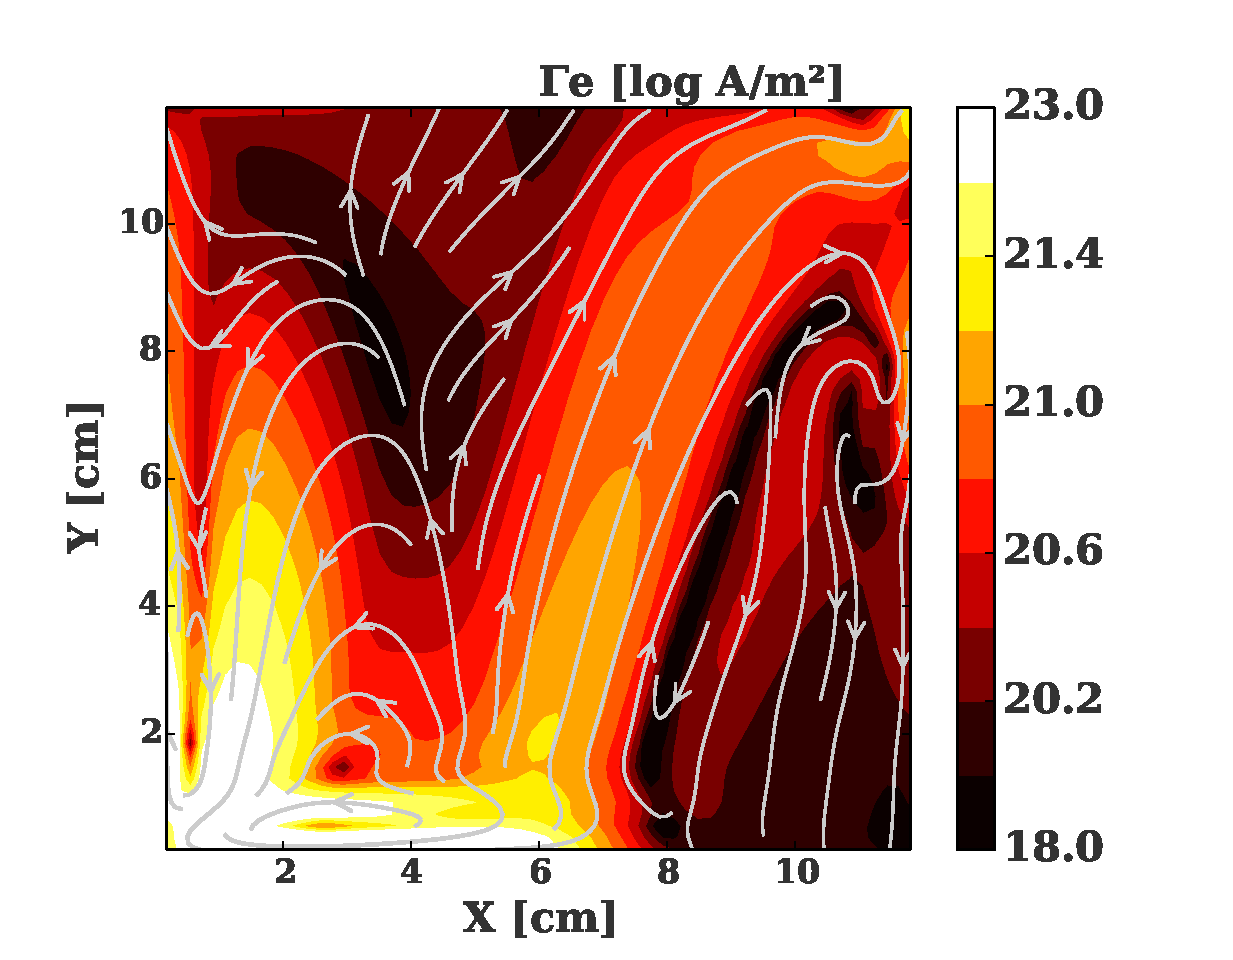
\includegraphics[height=6cm]{figures/4-PegasesCarteFluxEBase.eps}}
    \caption{Densité de courant ionique \subref{4-PegasesCarteFluxEBase}~
    et électronique \subref{4-PegasesCarteFluxEBase}.}
    \label{4-PegasesCarteFlux}
\end{figure}

Dans la zone non
magnétisée, les ions issus de l'ionisation du gaz sont créés avec une vitesse
initiale quasiment nulle et tombent de façon rectiligne aux parois. Du côté
magnétisé, le flux augmente fortement puis diminue à travers le filtre (les
ions sont perdus le long des lignes), mais celui-ci n'a pas d'influence notoire
sur la trajectoire des particules.

Le flux électronique est quant à lui représentatif de la configuration du filtre
magnétique. On visualise bien le fort courant qui
remonte le long de la direction $y$. Ce comportement, à l'origine de l'asymétrie
générale du plasma, se retrouve dans d'autres sources utilisant un filtre
magnétique, notamment dans la sources d'ions négatifs de
Garching~\parencite{Fantz} et a été modélisé dans ce contexte à travers
différents modèles, fluides et cinétiques~\parencite{PIC2D,PIC3D,MAGMA}.

Contrairement aux propulseurs à
effet Hall, dans lesquels le courant de Hall est confiné le long d'une
direction périodique, dans le cas de
la configuration filtre ce courant est bloqué et donne naissance à un réel effet 
Hall, ressemblant à celui que l'on connaît dans les solides : un courant
électrique traversant un matériau baignant dans un champ magnétique engendre une tension
perpendiculaire à celui-ci. Seulement, dans les plasmas, ce n'est pas juste une
tension qui se met en place mais tout le plasma qui se polarise et se déforme
sous la contrainte du champ magnétique pour faire passer le courant.

On peut remarquer
deux autres phénomènes, moins détaillés dans la littérature : tout d'abord il
faut noter que le flux le plus important se situe dans la zone non magnétisée au
niveau de la paroi dans la région que nous appellerons basse de la source (en
$y\sim\,$0~cm).
La figure~\ref{4-PegasesCarteFluxEBase} montre que le flux électronique
traversant le filtre prend sa source dans la région basse du filtre, qui
s'alimente à son tour en attirant le plasma le long de la paroi.
Le deuxième point concerne la région en aval du filtre, où l'on observe que le
flux électronique traverse le domaine en sens inverse, une partie de celui-ci franchissant même à nouveau
la barrière magnétique au niveau de la paroi opposée.

\subsection{Étude paramétrique}
Dans cette partie, nous
réalisons une étude paramétrique sur les paramètres susceptibles
d'influencer le comportement du plasma dans le propulseur. Nous faisons varier
la pression de gaz, le profil de dépôt de puissance ainsi que la forme et
l'intensité du champ magnétique dans un plasma d'argon pur. Les paramètres et
les plages de valeurs qui ont été regardés correspondent à ceux testés par
Jérôme Bredin pendant une étude sur la chute de température électronique en
présence d'un champ magnétique non-uniforme~\parencite{Bredin}\footnote{Nous ne
montrons cependant pas les résultats expérimentaux, ceux-ci provenant de
communications privées et n'ayant pas encore été parus. Nous essayons tout de
même de nous placer au plus près des conditions expérimentales.}, nous donnant
ainsi une base intéressante pour tester et discuter les résultats du modèle.

Dans ces expériences, la
grille d'extraction est enlevée, la source étant reliée à un grand volume
diminuant l'expansion spatiale du plasma. Pour nous placer au plus près des
conditions expérimentales, le domaine est allongé dans
la direction $x$ jusqu'à une longueur de 18~cm. Les parois sont quant à elle
choisies diélectriques. Les profils sont pris dans la direction $x$, au niveau
du milieu de la source (en $y\,=$ 6~cm) et il faut donc garder en tête la
présence de l'asymétrie générale du plasma, qui n'apparaît pas sur ces coupes.
	
\subsubsection{Scan en pression}
Nous regardons tout d'abord l'effet de la pression du gaz, choisie
successivement à 1 mTorr, 10 mTorr et 100 mTorr, sur le transport du plasma.
Les paramètres des simulations sont rappelés dans le
	tableau~\ref{4-PegasesScanPreParam}. 

\begin{minipage}{\textwidth}
\footnotesize\centering
\ra{1.3}
\begin{tabular}{lcclc}\toprule
\multicolumn{5}{c}{\bf Paramètres}\\
\midrule 
Parois & Isolantes &&$L_x$, $L_y$, $L_z$  & 18cm, 12cm,
8cm\\
$\mathcal{P}_\text{ext}$&250W&&$l_\mathcal{S}$, $x_\mathcal{S}$&2cm, 0cm\\
$B$&250G&&$l_B$, $x_B$&2.5cm, 7.5cm\\
\textbf{gaz (Ar)} & \textbf{1--100 mTorr}&&$\Delta t$, $\Delta x$&10$^{-8}$s,
1mm\\
\bottomrule
\end{tabular}
\captionof{table}{Paramètres de la simulation.}\label{4-PegasesScanPreParam}
\end{minipage}	
	
	La
	figure~\ref{4-pegasesCompPressDenProfile} montre une comparaison des profils
	de densité. À 100~mTorr, la densité du plasma atteint 10$^{18}$~m$^{-3}$ puis
	décroît exponentiellement jusqu'à $x\sim\,$ 11~cm vers la fin de la région
	du filtre. 
	La température électronique, dont le profil est montré
	figure~\ref{4-pegasesCompPressTempProfile}, reste approximativement égale à
	2~eV et n'est impactée par le filtre magnétique qu'après son maximum, en $x\sim\,$ 7.5~cm.
\begin{figure}[!htbp]
  \centering
    \subfigure[]{\label{4-pegasesCompPressDenProfile}
    
\includegraphics[height=5cm]{figures/4-pegasesCompPressDenProfile.eps}}
    \subfigure[]{\label{4-pegasesCompPressTempProfile}
    
\includegraphics[height=5cm]{figures/4-pegasesCompPressTempProfile.eps}}
    \caption{Profils de densité~\subref{4-pegasesCompPressDenProfile}~ et de
    température~\subref{4-pegasesCompPressTempProfile}~ pour trois pressions de
    gaz différentes, 1~mTorr, 10~mTorr et 100~mTorr.}
    \label{pegasesCompPressProfils}
\end{figure}
	La diminution de la pression a une influence sur plusieurs points :
	
	\begin{itemize}
	  \item la densité maximale du plasma baisse globalement dans la zone en amont
	  du filtre : 10$^{18}$~m$^{-3}$ à 100~mTor, 4.10$^{17}$~m$^{-3}$ à 10~mTorr et
	  2.10$^{17}$~m$^{-3}$ à 1~mTorr
	  \item de l'autre côté du filtre, la densité du plasma a au contraire
	  tendance à augmenter
	  \item la température évolue en sens inverse : avant le filtre, elle augmente
	  successivement de 2~eV (100~mTorr) à plus de 3~eV (10~mTorr) pour atteindre
	  un peu moins de 7~eV à basse pression (1~mTorr) 
	  \item la chute de température à travers le
	  filtre est bien plus importante à basse pression\footnote{On note cependant que le minimum de température n'est pas atteint exactement
au même niveau que dans les expériences, celles-ci le plaçant au centre de la
barrière magnétique, et le modèle le prédisant plutôt à la fin du filtre (cette
différence pouvant éventuellement être imputée à la géométrie du champ
magnétique, totalement rectiligne dans le modèle).}
	\end{itemize}
	


	\subsubsection{Variations du champ magnétique}
	
	Nous faisons maintenant varier l'intensité du champ magnétique en gardant une
	pression de gaz constante à 1~mTorr. La comparaison des profils pour des champs
	magnétiques d'intensité 50~G, 140~G et 250~G est présentée
	figure~\ref{4-pegasesCompMagProfile}. Le seul effet visible sur la
	figure~\ref{4-pegasesCompMagDenProfile} correspond à l'augmentation moyenne de
	densité dans la région du filtre qui passe de 8.10$^{16}$~m$^{-3}$ à un peu
	plus de 10$^{17}$~m$^{-3}$. À 250~G, le profil de densité forme un palier
	sur quelques centimètres.
	
	L'influence de l'augmentation de l'intensité du champ magnétique est bien moins
	visible sur le profil de température : on voit tout de même que $T_e$
	s'élève au niveau de la paroi en $x\,$=0~cm et que sa décroissance à travers le
	filtre s'effectue sur une plus courte distance. À 50~G, la température dans la
	région en aval du filtre est aux alentours de 2~eV, soit un peu plus haute que
	dans les cas à 140~G et 250~G.
	
\begin{figure}[!htbp]
  \centering
    \subfigure[]{\label{4-pegasesCompMagDenProfile}
    
\includegraphics[height=5cm]{figures/4-pegasesCompMagDenProfile.eps}}
    \subfigure[]{\label{4-pegasesCompMagTempProfile}
    
\includegraphics[height=5cm]{figures/4-pegasesCompMagTempProfile.eps}}
    \caption{Profils de densité \subref{4-pegasesCompMagTempProfile}~ et de
    température \subref{4-pegasesCompMagTempProfile}~ pour trois intensité de
    champ magnétique 50G, 140G et 250G.}
    \label{4-pegasesCompMagProfile}
\end{figure}

Au cours des différentes simulations, nous avons remarqué que les profils
étaient plutôt sensibles aux tailles (largeurs) du filtre magnétique et de la
forme du profil de puissance injectée\footnote{Dans les expérimentations
effectuées au LPP, l'augmentation de l'intensité du champ magnétique est accompagnée d'un
élargissement de la largeur du filtre. Nous testons donc aussi l'influence de
ce paramètre.}.
Pour confirmer ces observations, faisons varier à la fois $l_\mathcal{S}$ la
largeur de dépôt d'énergie et $l_B$ la largeur de la barrière pour deux intensités de
champ magnétique puis comparons la densité maximale et la température des
électrons après le filtre. On voit dans le tableau \ref{4-pegasesCompLargeurs}
que quand le filtre est plus long, la densité augmente et la température baisse
de façon plus prononcée.
De l'autre côté, quand l'énergie est déposée sur une plus grande distance, la
densité a plutôt tendance à diminuer tandis qu'après la barrière, la
température électronique remonte.

\begin{table}
\footnotesize\centering
\ra{1.3}
\begin{tabular}{@{}ccccccc@{}}\toprule
\bfseries B&&\multicolumn{2}{c}{$l_B=2cm$} && \multicolumn{2}{c}{$l_B=4cm$}\\
\cmidrule{3-4} \cmidrule{6-7}
&& $n (m^{-3})$ & $\min T_e (eV)$ && $n (m^{-3})$ & $\min T_e (eV)$\\
\midrule 
250G\\
\scriptsize $l_\mathcal{S}=2cm$ &&\bfseries\scriptsize 1.58
10\textsuperscript{17}&\bfseries\scriptsize 0.91&&\scriptsize 2.3
10\textsuperscript{17}&\scriptsize 0.73
\\
\scriptsize $l_\mathcal{S}=4cm$  &&\scriptsize 1.4 10\textsuperscript{17}
&\scriptsize 2.08&&\scriptsize 2 10\textsuperscript{17}&\scriptsize 1.38\\
140G\\
\scriptsize $l_\mathcal{S}=cm$ &&\scriptsize 1.57 10\textsuperscript{17}
&\scriptsize 1.27&&\scriptsize 1.96 10\textsuperscript{17}&\scriptsize 0.98 \\
\scriptsize $l_\mathcal{S}=4cm$  &&\scriptsize 1.39 10\textsuperscript{17}
&\scriptsize 2.36&&\bfseries\scriptsize 1.75 10\textsuperscript{17}&\bfseries\scriptsize
1.6\\
\bottomrule
\end{tabular}
\caption{Tableau comparatif présentant la densité maximale du plasma ainsi que
la température électronique après le filtre magnétique pour des largeurs de
source d'énergie $l_S$ et de filtre magnétique $l_B$ différentes.}
\label{4-pegasesCompLargeurs}
\end{table}

Quand on compare les résultats de MAGNIS avec les mesures du LPP, les 
profils de densité sont plutôt concordants lors des changements de pression. Les
tests sur la variation de l'intensité du champ magnétique seule montrent
au contraire peu de modifications significatives sur le transport, ce qui n'est
pas le cas avec les expériences.

Cependant, dans les mesures réalisées sur PEGASES, le filtre magnétique est
respectivement de largeur 4 cm et 2 cm dans les cas à 140 G et 250 G. Dans le
tableau~\ref{4-pegasesCompLargeurs}, si l'on ne retient que ces deux
combinaisons d'intensité et de largeur de champ, les valeurs se rapprochant le
plus des données expérimentales (en gras dans le tableau) correspondent à
une largeur de source plus petite dans le cas fortement magnétisé et
inversement à une largeur de puissance déposée plus grande quand le champ
magnétique est plus étendu. L'influence de la taille de la zone de chauffage
n'est donc pas négligeable dans le cas des sources d'ions et semble de plus
varier en fonction de la configuration magnétique.

\subsection{Transport du courant dans le cas de parois conductrices et d'un bias
appliqué}

La suite de cette étude porte sur le cas de parois
conductrices. Dans cette configuration, représentative de
l'un des modes de fonctionnement de PEGASES ainsi que de nombreuses
expérimentations, l'application d'un bias positif sur la grille d'extraction afin d'extraire un
courant d'ions négatifs modifie de manière conséquente les boucles de
courant dans le plasma (dans la source de Garching, on joue sur le bias pour
optimiser les flux). Le transport du courant est régit par l'équation de
conservation du courant :

\begin{equation}
\nabla\cdot\mathbf j=\nabla_\para\cdot \mathbf j_\para +\nabla_\perp\cdot
\mathbf j_\perp
\end{equation}

Quand les parois de la source sont
isolantes, aucun courant ne peut entrer ou sortir du plasma. En l'absence de
champ magnétique, il n'y a alors que peu de contraintes sur celui-ci, ce qui le
laisse quasiment nul dans l'ensemble de la source. Avec des parois conductrices,
on peut au contraire forcer un courant à travers le plasma en ajustant les
conditions aux limites (en appliquant un bias sur l'une des parois).
Même dans un cas simple sans champ magnétique appliqué, le courant peut alors
former des vortex (tourbillons) et se reboucler dans les parois
conductrices (effet court-circuit découvert par Simon~\parencite{Simon55}).

L'effet Simon est particulièrement déterminant pour le transport
global du plasma en présence d'un champ magnétique ; les électrons, qui auront plutôt
tendance à faire passer le courant par les parois qui
interceptent les lignes de champ magnétique, court-circuitent l'intérieur du
plasma. La gaine au bout des lignes de champ joue alors un rôle crucial dans
l'évolution du potentiel, et ce jusqu'au c\oe{}ur de la source. À basse
pression, les solutions deviennent instationnaires, et le transport change
radicalement de nature, devenant instable avec des phénomènes instationnaires
et réguliers.
	
\subsubsection{Influence du champ magnétique}
Dans les sources d'ions utilisant un filtre magnétique, on sait que le flux
d'électrons est le principal responsable de l'inhomogénéité
de densité observée~\parencite{PIC2D,PIC3D}. Nous regardons donc son
comportement à travers la variation de l'intensité du champ magnétique et d'un
bias appliqué à la grille d'extraction (sur la paroi droite du domaine de
simulation, voir figure~\ref{4-pegasesSimDomain}).
Les paramètres des simulations sont rappelés dans le tableau~\ref{4-PegasesScanMagParam}.
Notons le courant total d'électron récupéré sur la grille d'extraction par :

\begin{equation}
I_e=\int_S j_e\text{dS}
\end{equation}
\begin{minipage}{\textwidth}
\footnotesize\centering
\ra{1.3}
\begin{tabular}{lcclc}\toprule
\multicolumn{5}{c}{\bf Paramètres}\\
\midrule 
Parois & Conductrices &&$L_x$, $L_y$, $L_z$  & 12cm, 12cm,
8cm\\
$\mathcal{P}_\text{ext}$&250W&&$l_\mathcal{S}$, $x_\mathcal{S}$&2cm, 0cm\\
$B$&\textbf{0--250 G}&&$l_B$, $x_B$&2.5cm, 7.5cm\\
$\Phi_w$ & \textbf{0--20 V}&&gaz (Ar) & 1 mTorr\\
\bottomrule
\end{tabular}
\captionof{table}{Paramètres de la simulation.
Nous faisons varier l'intensité du champ
magnétique de 0~G à 250~G et le bias appliqué de
0~V à 20~V.}\label{4-PegasesScanMagParam}
\end{minipage}

avec $j_e$ représentant la densité de courant électronique sur la paroi. $I_e$
est théoriquement réduit d'un facteur en $1/B^2$ à travers le filtre dans une
analyse unidimensionnelle (ne tenant pas compte de la direction de dérive $y$).
On peut voir sur la figure~\ref{pegasesVarMagCourantParoi} le courant total
$I_e$ récupéré au niveau de la grille d'extraction (sur le bord droit du
domaine) : sans bias appliqué, $I_e$ suit à peu près cette loi d'échelle en
$1/B^2$. Cependant, quand le bias augmente, on voit que le $I_e$ commence plutôt
à suivre une loi en $1/B$. Cette variation en $1/B$ est généralement prise
comme la signature de la présence d'un transport anormal.

Pourtant, dans ces sources, le transport reste classique et la raison de cette
augmentation significative doit être recherchée dans les effets
induits par les dérives  magnétiques. Actuellement, même si les tentatives d'explications
s'accordent sur la traversée du filtre des électrons via la forte dérive ExB à proximité de la
gaine, la déviation d'origine du flux électronique en face du filtre reste à
l'origine de nombreux débats.

\begin{figure}[!htbp]
	\centering
	
\includegraphics[width=0.6\textwidth]{figures/4-pegasesVarMagCourantParoi.eps}
	{\caption{Courant total d'électrons récupéré sur la grille d'extraction $I_e$
	en fonction de l'intensité du filtre magnétique pour trois voltages appliqués (0 V, 10 V et 20 V). }
	\label{pegasesVarMagCourantParoi}}
	\end{figure}

\subsubsection{Le flux électronique magnétisé}

Attardons nous donc sur le flux électronique, à travers l'augmentation
progressive de l'intensité du champ magnétique. La
figure~\ref{4-pegasesfluxElectronique} représente une comparaison croisée du
flux d'électrons pour un champ magnétique variant de 0 G à 500 G et trois bias
différents de 0 V, 10 V et 20 V appliqués à la grille d'extraction de la source. 

 \begin{figure}[!htbp]
	\centering
	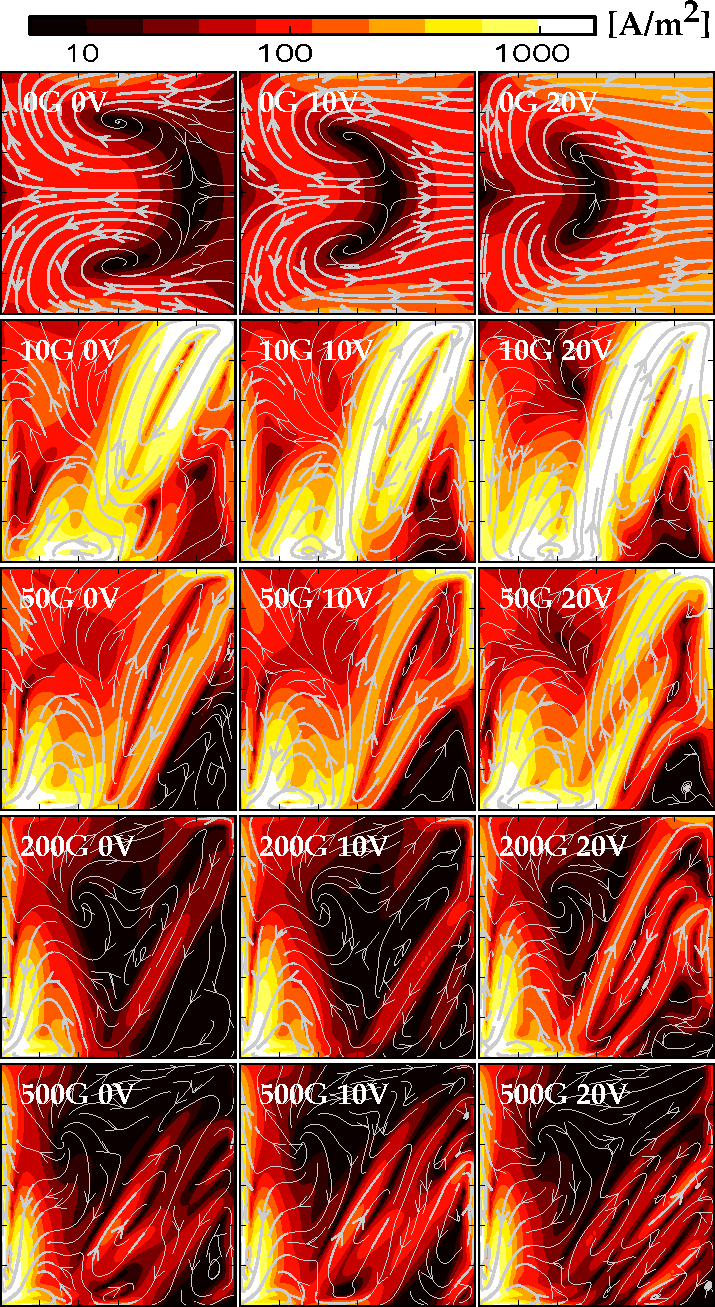
\includegraphics[width=0.85\textwidth]{figures/4-pegasesfluxElectronique.pdf}
	{\caption{Flux électronique à travers le filtre magnétique sur une plage
	allant de 0 G à 500 G pour trois voltages appliqués sur la grille
	d'extraction (sur le bord droit du domaine) différents 0~V, 10~V et 20~V.}
	\label{4-pegasesfluxElectronique}}
	\end{figure}

Les trois premières cartes, en l'absence de filtre magnétique, montrent la
situation initiale pour les trois différents voltages. Basiquement, on observe
que l'application du bias attire le flux électronique qui peut alors atteindre
dans le plasma une densité de courant de l'ordre de $\sim$10$^2$ A/m$^2$ et que
le flux à la paroi est uniforme\footnote{Cette
situation, bien que basique, est déjà intrigante en soi : le flux électronique
forme des vortex en dehors de la région d'ionisation et remonte le long des
gradient de densité. Ce phénomène est hors de contexte du présent
manuscrit mais mérite tout de même d'être signalé, étant totalement absent de
la littérature.
Des simulations PIC ont par ailleurs montré un comportement
similaire~\parencite{PIC3D}.}.

L'application d'un filtre magnétique, même à faible intensité de champ, modifie
complètement le flux électronique : la densité de courant devient asymétrique et
décuple d'intensité dans le bas de la région d'ionisation. À 10 G, la
température électronique est de l'ordre de 5 eV, donnant un rayon de Larmor
électronique d'environ 5 mm. Les électrons sont déjà magnétisés et ne peuvent
traverser le filtre qu'au niveau de la paroi située en $y\,$=12 cm. Le flux
d'électrons se sépare ensuite pour rejoindre les ions qui ont traversé la
barrière sans perturbation, une partie plus ou moins importante allant à la
paroi en fonction du bias et l'autre traversant le domaine en sens inverse
jusqu'à atteindre la paroi en $y\,$= 0 cm.

À 50 G, l'intensité du courant électronique reste importante et un phénomène de
circulation des électrons autour de la barrière magnétique devient plus clair.
L'application du bias montre aussi que le flux est dévié et longe la grille
d'extraction sur quelques centimètres en direction de la partie basse du filtre.
À 200 G et sans bias appliqué, le flux électronique est fortement réduit à travers la barrière et change encore de
forme : le premier courant qui remontait le long du champ magnétique devient
moins important que le flux de retour en bas de la barrière. L'application d'un
bias ou l'augmentation de l'intensité du champ magnétique mène alors à
l'apparition d'un phénomène instable que nous allons regarder plus en détail dans la partie suivante.

Plus généralement, sur l'ensemble des cas présentés avec $B\neq\,$0, on remarque
que le bias ne change pas radicalement les profils du flux.

\subsection{Phénomènes intermittents, instabilités}
À faible champ magnétique ou à pression suffisamment élevée, les solutions
obtenues par MAGNIS sont stationnaires.
Cependant, lorsque la pression diminue, le transport collisionnel n'est plus
dominant et des phénomènes instables, caractéristiques des plasmas
magnétisés, peuvent apparaître et affecter toute la dynamique du système. 
 
\subsubsection{Vagues ioniques}
La première instabilité que l'on voit apparaître est illustrée
figure~\ref{4-PegasesCarteDensiteWaves}. À intervalles réguliers, des bouffées
de plasma traversent le filtre magnétique à des vitesses de l'ordre de la
vitesse de Bohm du système.
La direction de propagation est perpendiculaire au front de densité, à
l'oblique entre le champ magnétique et son gradient. Sans bias et à une
pression de gaz de 1~mTorr, les fronts de densité apparaissent à une fréquence
d'environ 120kHz et se déplacent à une vitesse approximative de 2.10$^3$
m.s$\puissance{-1}$.
 
\begin{figure}[!htbp] 
  \centering
    \subfigure[]{\label{4-PegasesCarteDensiteWaves}
    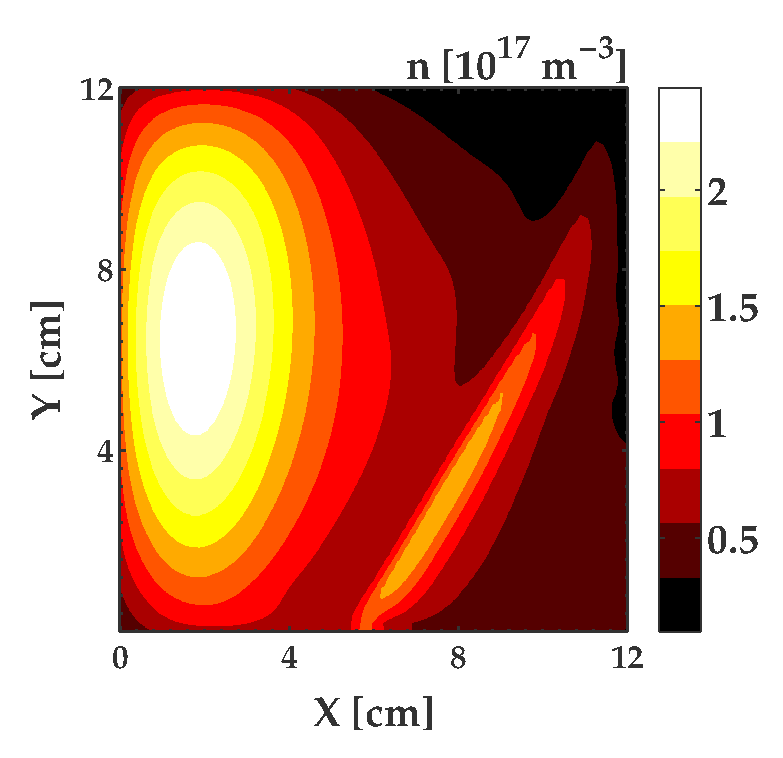
\includegraphics[height=5cm]{figures/4-PegasesCarteDensiteWave.eps}}
    \subfigure[]{\label{4-PegasesCarteViSurTeVarBias}
    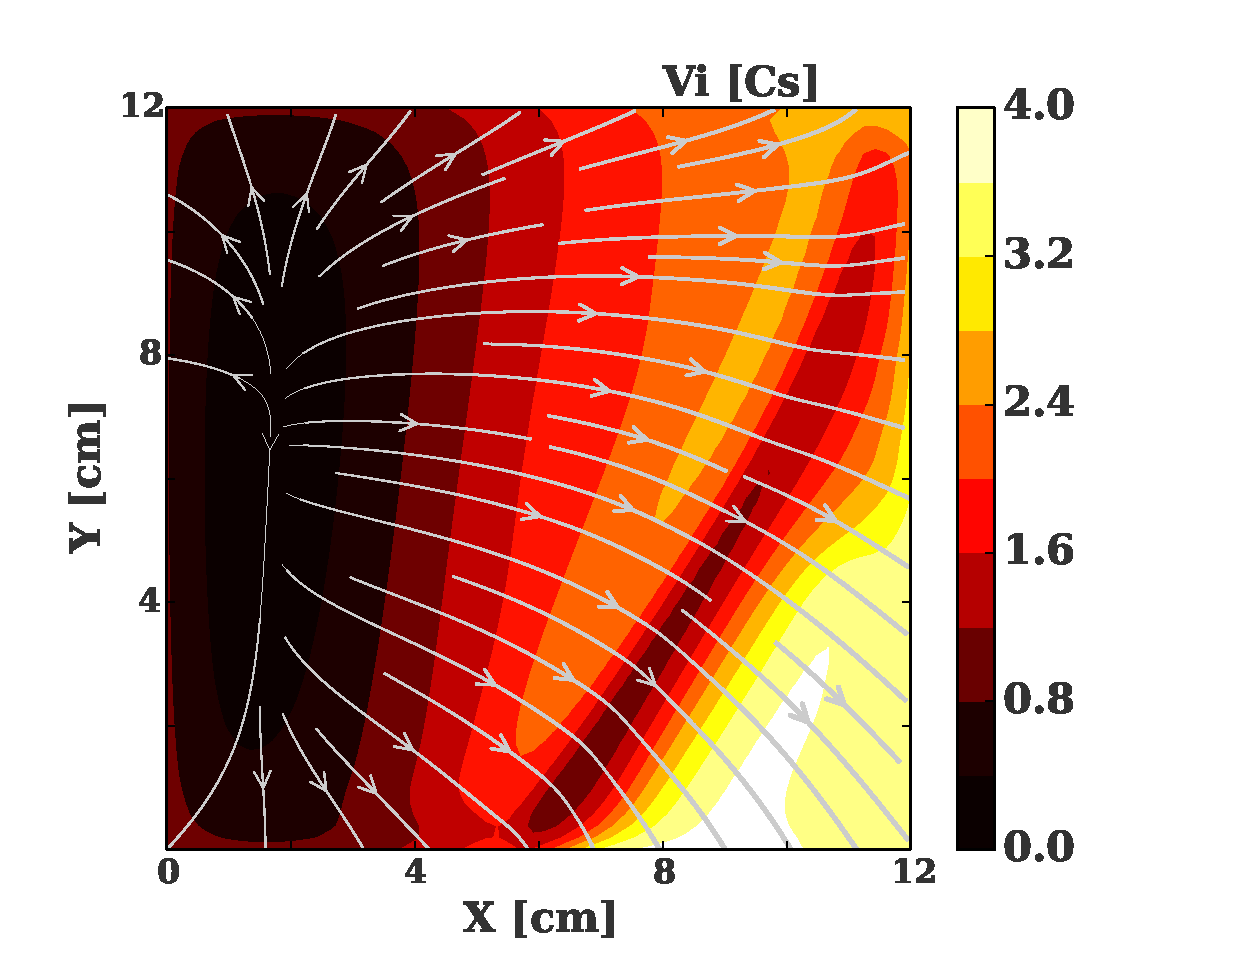
\includegraphics[height=5cm]{figures/4-PegasesCarteViSurTeVarBias.eps}}
    \caption{Cartes de la densité plasma~\subref{4-PegasesCarteDensiteWaves}~ et
    de vitesse ionique rapportée à la
    vitesse de Bohm locale
    $c_s=\sqrt{T_e/m_i}$~\subref{4-PegasesCarteViSurTeVarBias}~ pour un champ
    magnétique de 250 G, une densité d'argon de 1~mTorr et un bias appliqué de
    20V.}
    \label{4-PegasesVaguesIoniques}
\end{figure}
 
 La figure~\ref{4-PegasesCarteViSurTeVarBias} représente la vitesse ionique
 rapportée à la vitesse de Bohm, i.e. le nombre de Mach de
 l'écoulement ionique. On voit tout d'abord qu'une grande partie du domaine est
 occupée par des ions dont la vitesse dépasse la vitesse de Bohm locale. En
 effet, les ions franchissent le seuil $v_i=c_s$ (Mach1) le long du gradient de
 température, à $T_e\sim\,$5 eV puis accélèrent encore jusqu'à atteindre
 $v_i=2c_s$ (Mach2) avant le front de densité. La vitesse décroît ensuite lors
 de la traversée de la bouffée, tout en restant de l'ordre de la vitesse de
 Bohm.
 
 La vitesse de phase $v_\phi$ calculée ($v_\phi\sim\,$2.10$^3$
 m.s$\puissance{-1}$) , représentative de la propagation de la bouffée, est inférieure à la
 vitesse des particules la constituant ($u_i\sim\,$4.10$^3$
 m.s$\puissance{-1}$). Très naïvement, ce phénomène fait penser aux phénomènes
 de compression-décompression liés aux ondes soniques dans les gaz
 classiques, où le front de densité serait l'onde acoustique
 résultante du passage des ions supersoniques. En supposant que la vitesse de
 propagation de l'onde est caractéristique de cette transition (dans
 l'analogie, les ondes sonores se déplacent à la vitesse du son), il est
 tentant de définir la température correspondante à $v_\phi$ :
 
 \begin{equation}
 	v_\phi=c_{s}=\sqrt{\frac{T_e}{m_i}}\simeq 2.2\;10^{3}\,\text{m.s}^{-1}
 	\Leftrightarrow T_e\simeq 2\,\text{eV}
 \end{equation}
 
 Quelques propriétés peuvent être immédiatement dégagées. L'apparition de cette
 instabilité et certaines de ses particularités sont directement reliées au
 gradient de température électronique et au terme d'inertie :
 
 \begin{itemize}
   	\item les solutions du modèle quand le terme inertiel d'advection est
	négligé sont stables ;
   \item quand on ne résout pas l'équation d'énergie, avec une température
   électronique uniforme, le plasma redevient stable et s'étend dans le filtre
   dans la direction du flux d'électrons transverse ;
   \item la direction des fronts d'ondes est fortement corrélée au gradient
   de température.
\end{itemize}

La réponse à la polarisation de la grille d'extraction est aussi une
caractéristique intéressante de ce phénomène. Les
figures~\ref{4-PegasesCarteDensiteVarBiasWave}\subref{4-PegasesCarteDensiteVarBias1}, \subref{4-PegasesCarteDensiteVarBias2}
et~\subref{4-PegasesCarteDensiteVarBias3} illustrent cet effet en partie : la
dynamique des fronts, de vitesse de phase $v_\phi$ approximativement constante à
0~V, se décompose en deux temps après l'application d'un faible voltage. Les
fronts ralentissent au niveau du maximum du filtre magnétique, augmentent en densité, puis sont
propulsés vers les parois après un certain temps de latence. À 30~V, en
l'absence de champ accélérateur, un bras de plasma se forme en travers du
filtre, de densité équivalente à celle du plasma de la région d'ionisation.
	
	\begin{figure}[!htbp]
  \centering
    \subfigure[]{\label{4-PegasesCarteDensiteVarBias1}
    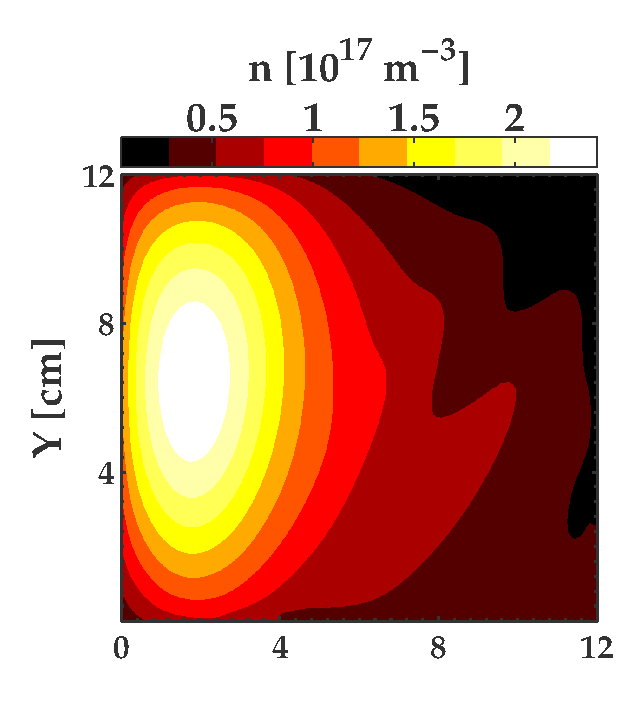
\includegraphics[height=6cm]{figures/4-PegasesCarteDensiteVarBias1.eps}}
    \subfigure[]{\label{4-PegasesCarteDensiteVarBias2}
    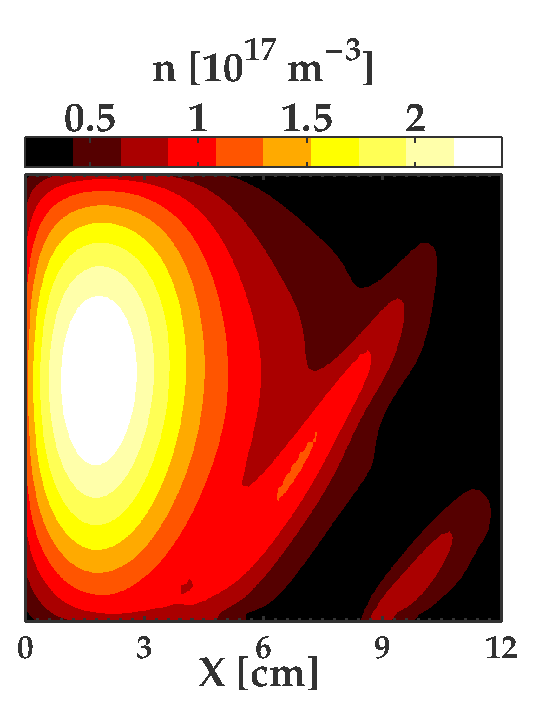
\includegraphics[height=6cm]{figures/4-PegasesCarteDensiteVarBias2.eps}}
    \subfigure[]{\label{4-PegasesCarteDensiteVarBias3}
    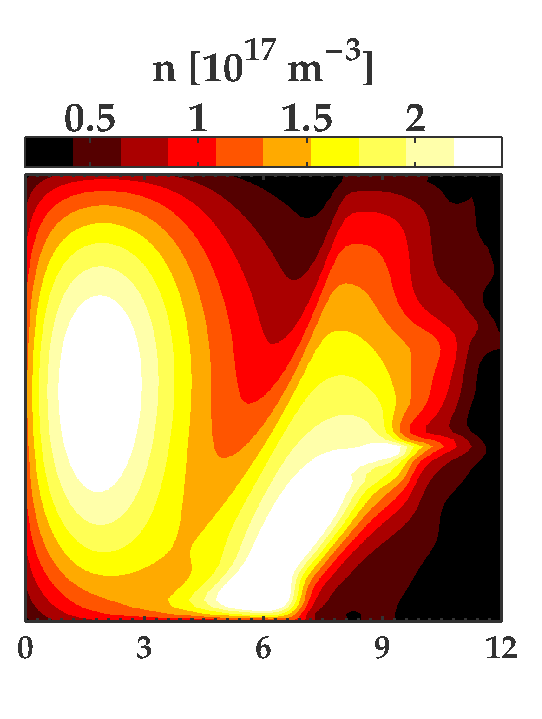
\includegraphics[height=6cm]{figures/4-PegasesCarteDensiteVarBias3.eps}}
    \caption{Cartes de densité pour
    trois bias appliqués : 0V\subref{4-PegasesCarteDensiteVarBias1},
    10V\subref{4-PegasesCarteDensiteVarBias2} et
    30V\subref{4-PegasesCarteDensiteVarBias3}.}
    \label{4-PegasesCarteDensiteVarBiasWave}
\end{figure}

On peut maintenant préciser la forme du flux électronique 
dans les cas fortement magnétisés de la
figure~\ref{4-pegasesfluxElectronique}. Un champ électrique apparaît
entre les fronts de densité, et se combine au filtre
magnétique pour faire naître un mouvement de dérive du type ExB, amplifiant le
transport des électrons au travers de la barrière. 

Nous avons fait varier le maillage spatial de 32 points à 512
points. Plus le maillage se raffine, plus la fréquence des bouffées augmente.
Les fronts se rapprochent et deviennent plus nombreux, mais gardent toujours la
même vitesse. Nous avons essayé de jouer avec les paramètres de la simulation
pour faire disparaître ces instabilités, mais sans succès, celles-ci
restant toujours présentes.
Des simulations PIC, récemment lancées au GREPHE sur une géométrie similaire
à notre configuration, semblent aussi montrer un comportement similaire.

La réalité physique de
ce phénomène n'est pas évidente et cette
dépendance quantitative au maillage rend la caractérisation complète de
l'instabilité assez difficile à réaliser.  
La présence d'ions supersoniques ne serait
pourtant pas surprenante, étant donné les gradients extrêmes, la très faible
température électronique après le filtre, et la forte tension retenant le flux
ionique.

	\subsubsection{Peigne de densité}
	À plus haute pression (10 mTorr et 100 mTorr), l'application d'un bias positif
	à la grille d'extraction révèle une autre instabilité qui prend la forme d'un
	"peigne" (cf.
	figure~\ref{4-PegasesCarteDensiteVarBias5}). Les pics de densités ne sont pas
	stationnaires mais se déplacent dans le sens des $y$ croissant, c'est à dire
	dans la direction de la dérive.
	On peut aussi la voir apparaître :
	
	\begin{itemize}
	  \item le long des fronts de densité
	  \item au niveau des parois
	  \item dans des simulations isothermes
	  \item dans un champ magnétique uniforme (cas de la colonne de plasma)
	\end{itemize}

	\begin{figure}[!htbp]
  \centering
    \subfigure[]{\label{4-PegasesCarteDensiteVarBias5}
    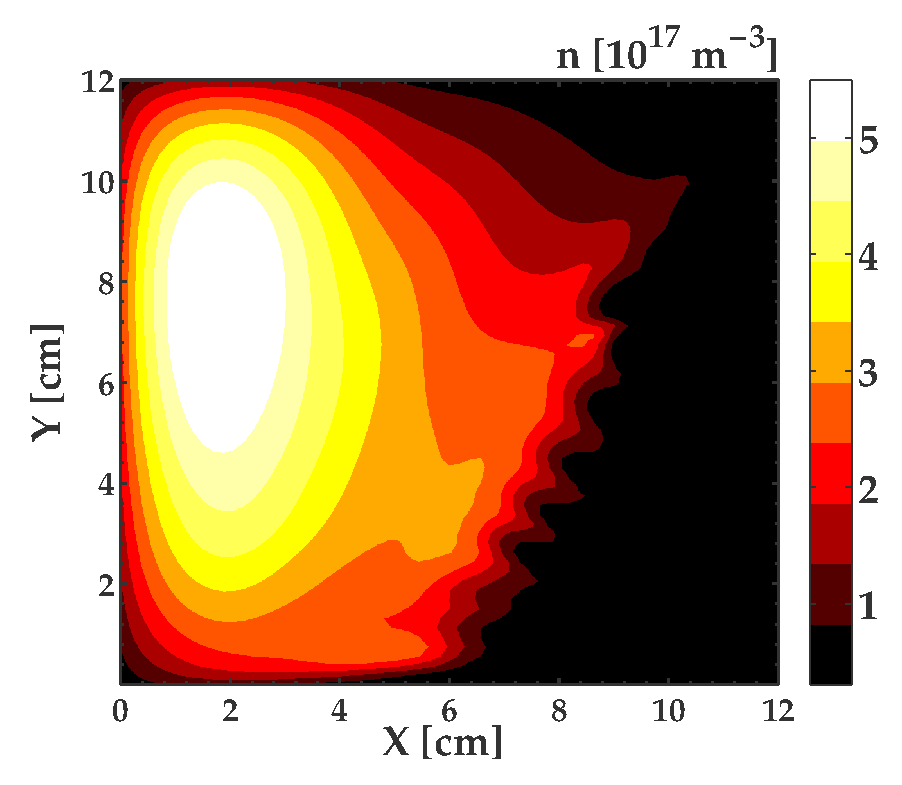
\includegraphics[height=6cm]{figures/4-PegasesCarteDensiteVarBias5.eps}}
    \subfigure[]{\label{4-PegasesCarteDensiteVarBiasPeriod}
    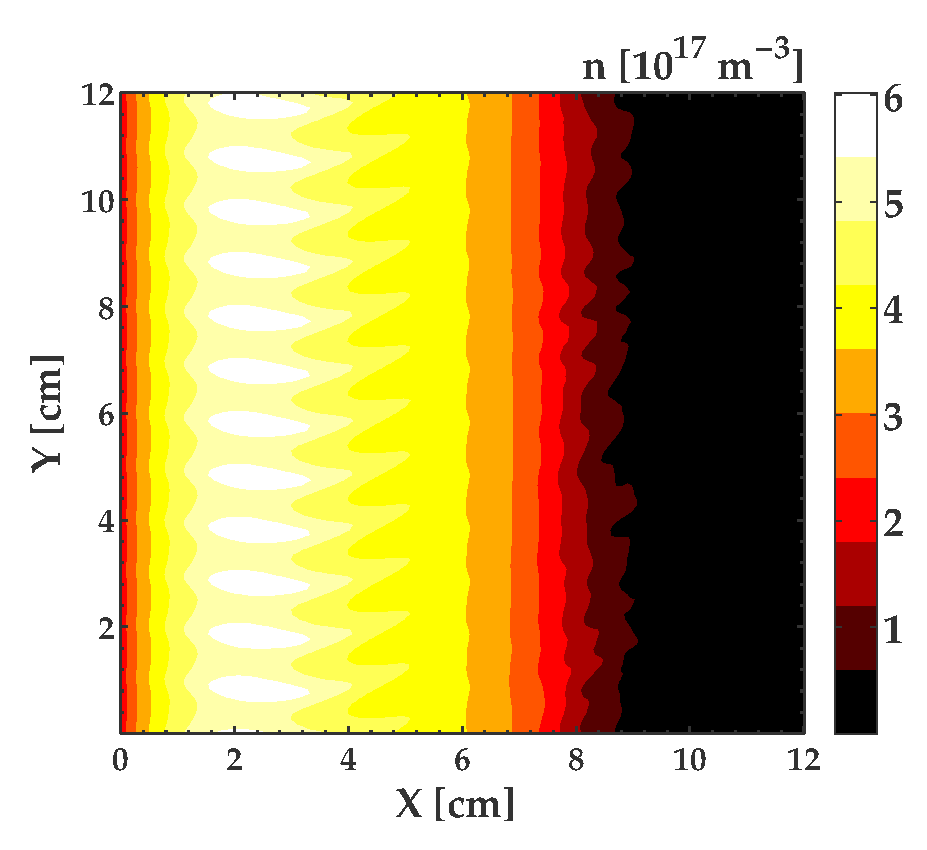
\includegraphics[height=6cm]{figures/4-PegasesCarteDensiteVarBiasPeriod.eps}}
    \caption{\subref{4-PegasesCarteDensiteVarBias5}~Carte de densité pour une
    pression de gaz de 10 mTorr et un bias de 30 V appliqué à la grille
    d'extraction. Des structures
    apparaissent à la limite du plasma et
    remontent le long du gradient de
    densité. \subref{4-PegasesCarteDensiteVarBiasPeriod}~Carte de densité pour les
    mêmes paramètres de simulation mais dans une géométrie périodique.}
    \label{4-PegasesCarteDensiteVarBias52}
\end{figure}

	L'instabilité est encore plus visible dans le cas d'une géométrie périodique
	en $y$ (i.e. dans lesquelles nous avons retiré les parois en $y\,$=0~cm et
	$y\,$=12~cm). Elle avait déjà été observée avec un code PIC2D sur
	une géométrie et avec des conditions plasmas similaires. La
	figure~\ref{4-PegasesCarteDensiteVarBiasPeriod} présente ce cas de test
	périodique :
	on observe que les pics se forment des deux côtés du filtre magnétique. À gauche, les
	structures se déplacent dans le sens des $y$ décroissants et à droite dans le
	sens des $y$ croissants.
	
	 Ce
	phénomène, qui se développe sur les bords du plasma et en présence d'un champ électrique important, rappelle
	les travaux de Simon~\parencite{Simon63} dans lesquels il démontre que l'état
	stationnaire peut devenir instable si le signe du produit du
	gradient de densité et du champ électrique est positif :
	
	\begin{equation}
		\nabla n\cdot \mathbf E>0
	\end{equation}
	
	Le champ électrique requis est dans la direction opposée à celle du champ
	électrique ambipolaire confinant usuellement les plasmas froids. Notre
	situation est cependant plus complexe que celle de Simon, qui porte
	sur un plasma isotherme et dont la géométrie est simplifiée par rapport à
	celle notre étude.

	Dans cette partie, nous avons tout d'abord donné des éléments pour
	valider le modèle dans une configuration de filtre magnétique. Nous avons ainsi
	montré que MAGNIS pouvait reproduire le comportement du flux électronique et
	l'inhomogénéité du plasma dans le plan perpendiculaire au champ
	magnétique. Nous avons aussi donné les premiers constats de la présence d'ions
	supersoniques et d'un transport instationnaire à travers le filtre.
	Malgré les problèmes de convergence numérique sur les instabilités, elles
	apparaissent dans différentes situations typiques et possèdent certaines
	caractéristiques invariables. Il est de plus très difficile de les supprimer en
	jouant sur les paramètres.
	
\section{Colonne de plasma magnétisée - Cybele}
\subsection{La configuration colonne magnétisée}
La colonne de plasma magnétisé est l'un des premiers
exemples que l'on rencontre dans les ouvrages traitant de la physique des
plasmas magnétisés. Dans cette géométrie très simple, le champ
magnétique est axial et uniforme, et le plasma, créé au centre de la colonne,
est très allongé dans la direction du champ magnétique. Celui-ci confine le
plasma et le met en rotation autour de l'axe central.

Dans cette géométrie, de nombreuses tentatives ont été entreprises pour
réduire le problème du transport du plasma dans le plan perpendiculaire à une
sorte de diffusion ambipolaire effective unidimensionnelle.
Cependant, même à très faible champ magnétique, le transport des ions et des
électrons est fondamentalement non ambipolaire : les courants, qui se referment
dans les parois aux extrémités des lignes de champ créé des court-circuits
tandis que dans le plan perpendiculaire se forment des vortex de courant, qui
stimulent significativement le transport transverse~\parencite{Gurevich}.

Il existe de nombreuses expérimentations en
configuration colonne magnétisée. Les plasmas y sont créés de différentes
manières, soit directement à l'intérieur de la colonne, soit par des sources situées à leurs
extrémités. Les modes de chauffage changent aussi en fonction des
expérimentations (filamentaire, RF, hélicon). Citons entre autres
:

\begin{itemize}
  \item Cybele au CEA de Cadarache, que nous décrirons plus en détail
  \item Mistral, au Piim de
  Marseille (chauffage extérieur par
  filaments, 40~cm de diamètre, 1.2~m de
  longueur, 2.5~kG)\parencite{Pierre, PierreExp, Brochard, Oldenburger}
  \item Mirabelle à Nancy (chauffage extérieur par
  filaments, $T_e$ à quelques eV, densité de
  10$^{15-17}$~m$^{-3}$, 33~cm de diamètre, 1.4~m de
  longueur, 1kG)~\parencite{Bousselin}
  \item NAGDIS-I et NAGDIS-II au Japon (source
  extérieure capacitive, 2.5~m de long, 18~cm de
  diamètre, $n_e\sim$10$^{19}$m$^{-3}$,
  $T_e\sim$5-10~eV, 2.5~kG)~\parencite{nishijimamodelling}
  \item CSDX (source hélicon, 15 cm de diamètre, 5 kW de puissance RF, champ
  magnétique de 2.4 kG)~\parencite{CSDX}
 \end{itemize}

Chacune dans ses objectifs de recherche particuliers, ces expérimentations
ont permis une amélioration de la théorie du transport magnétisé dans cette
géométrie de colonne en mesurant et analysant notamment : la rotation pas
toujours homogène du plasma, l'apparition de différents types
d'instabilités et, plus généralement, tous les mécanismes de transport qui se
mettent en place dans ces sources.
Les travaux ont de plus fourni une énorme quantité de mesures
expérimentales (sur des supports variant des sondes de Langmuir aux caméras
rapides) caractérisant les phénomènes de transport et les paramètres typiques
des plasmas obtenus sur une large gamme de conditions expérimentales
différentes.

Le test de MAGNIS sur cette configuration colonne de plasma magnétisé nous
donnera une validation supplémentaire pour le modèle. Dans l'ensemble des
sources précédemment citées, nous choisissons de simuler une configuration simplifiée de
Cybele. Ce choix a tout d'abord été motivé par les collaborations
développées autour de la problématique de l'injection
de neutres (IDN)\footnote{Dans le cadre du programme de recherche sur l'IDN,
le groupe GREPHE a déjà collaboré avec Alain Simonin qui développe Cybele au
CEA. J'ai notamment été invité à suivre les campagnes de caractérisation de
Cybele et à choisir un diagnostic à mettre en place (voir
figure~\ref{4-CybeleFourierSignal}).}.
La source Cybele est de plus de forme rectangulaire et donc parfaitement adaptée
au domaine de simulation de MAGNIS.

\subsection{La source d'ions négatifs Cybele}

Cybele, présentée sur la figure~\ref{4-cybelePhoto}, est une
source d'ions négatifs de dimension très allongée développée à l'IRFM
(CEA)~\cite{Simonin} dans le cadre de la recherche sur les systèmes d'IDN qui sont utilisés pour le chauffage et la génération de
courant dans les réacteurs de fusion par confinement magnétique\footnote{Le
principe d'un Injecteur De Neutres (IDN) est basé sur l'accélération d'ions à
très haute énergie, puis neutralisés afin de former un puissant faisceau de neutres.
Le faisceau est ensuite injecté au c\oe{}ur du réacteur pour déposer son énergie
directement dans le plasma. Pour ITER, les deux IDN devront fournir 17MW de
puissance chacun, en injectant 40A de D$\puissance{0}$ à
1MeV~\parencite{Hemsworth}.}.

\begin{figure}[!htbp]
  \centering
  \subfigure[]{\label{4-cybelePhoto}
    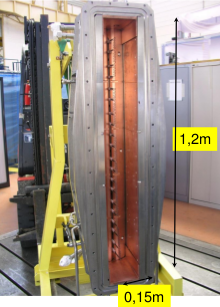
\includegraphics[height=8cm]{figures/4-cybelePhoto.png}}
    \subfigure[]{\label{4-CybelePhoto2}
    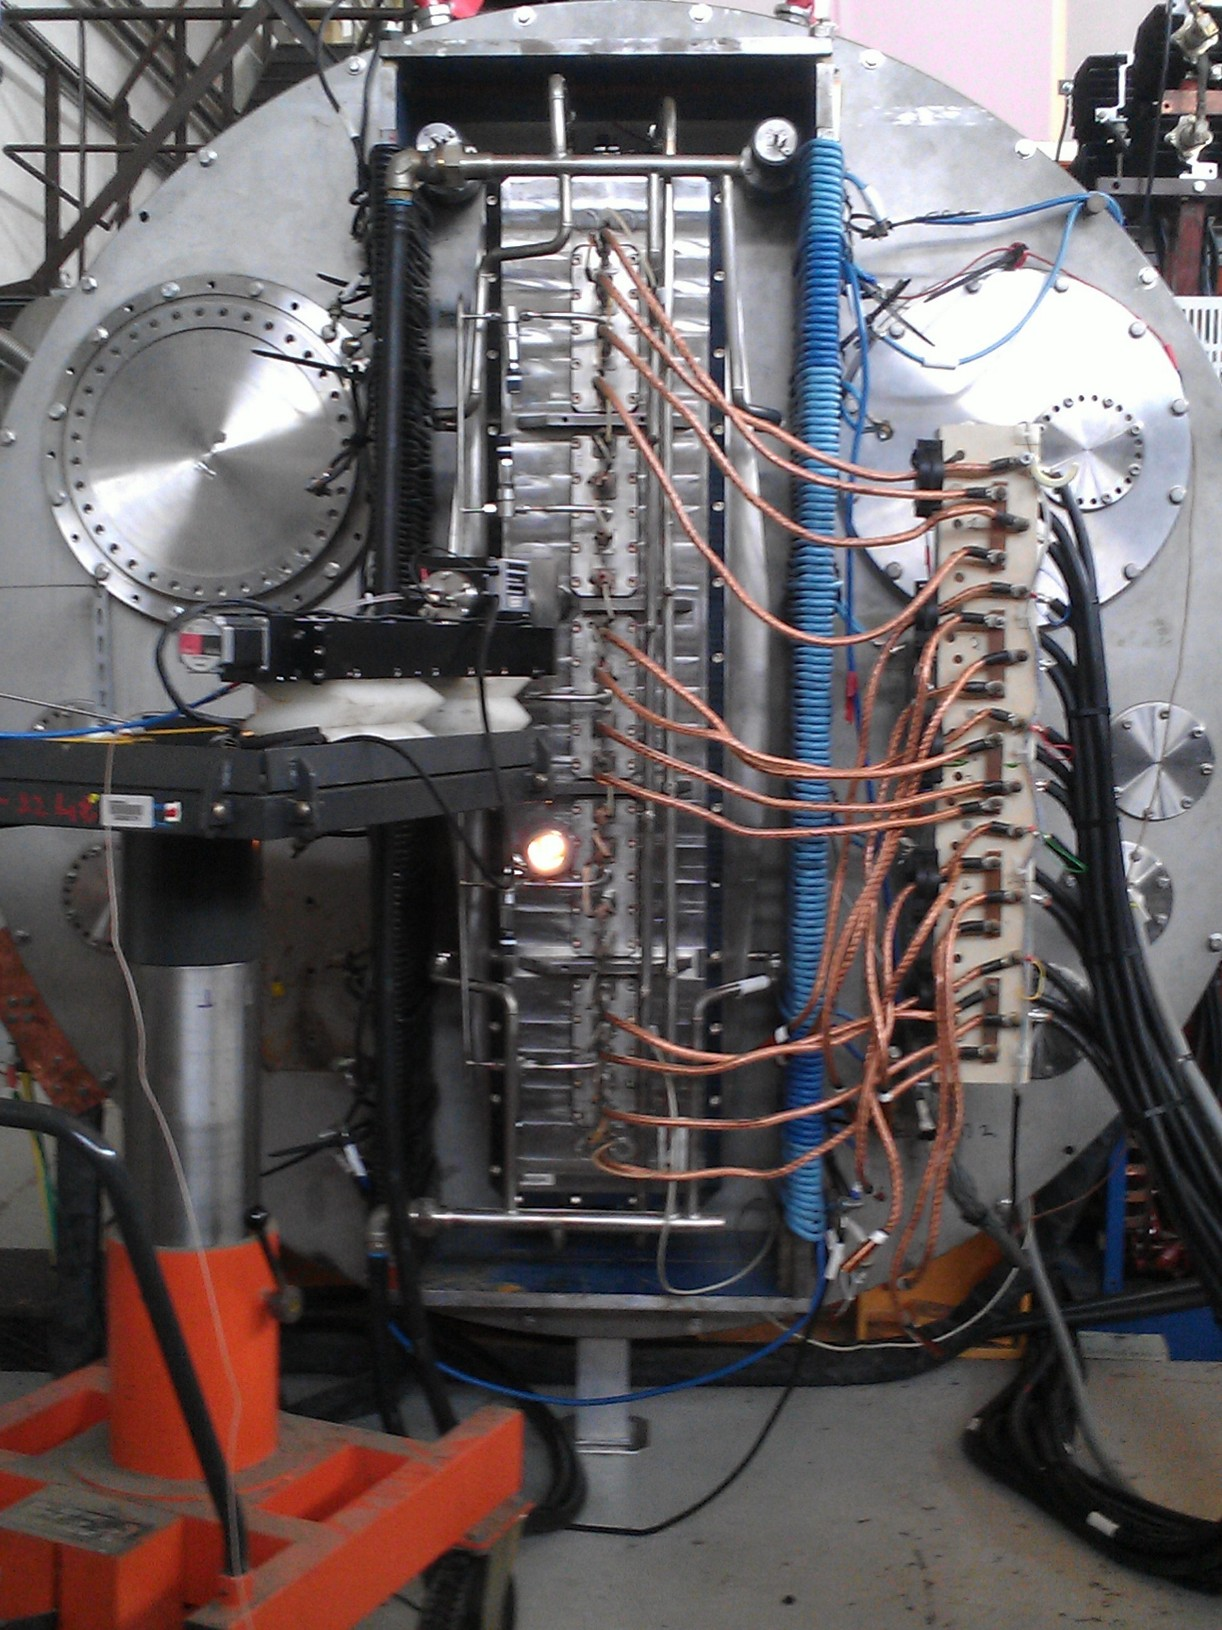
\includegraphics[height=8cm]{figures/4-CybelePhoto2.jpg}} 
    \caption{Photographies de la source d'ions négatifs Cybele en développement
    à l'IFRM de Cadarache~\parencite{SimoninHDR}. Le plasma est
    sondable radialement à partir du hublot (à travers lequel apparaît le
    plasma en jaune sur la photographie~\subref{4-CybelePhoto2}.)
    \label{4-cybelePhoto}} 
\end{figure}	

\begin{figure}[!htbp]
  \centering
    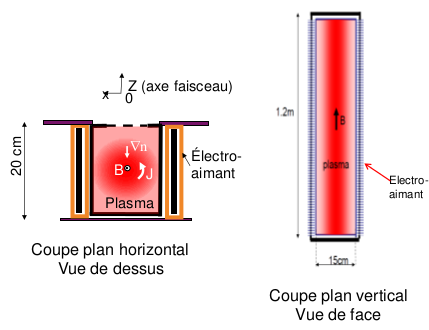
\includegraphics[height=8cm]{figures/4-cybeleSchema.png}
    \caption{Schémas de principe en coupe de Cybele~\parencite{SimoninHDR}. À
    gauche dans la vue de dessus, le champ magnétique est perpendiculaire au plan et confine le
plasma qui est créé au centre de la source. La vue de face montre quant à elle
la fine colonne de plasma, de densité homogène sur toute sa hauteur.
\label{4-cybeleSchema}}
\end{figure}	

Actuellement, les sources d'ions négatifs en amont des IDN se servent d'un champ
magnétique en configuration filtre pour refroidir les électrons (un schéma de la
source développée pour ITER est rappelé sur la figure~\ref{IPPIonSource2}).
Nous avons vu précédemment que cette configuration magnétique entraîne
dans ce type de sources de fortes inhomogénéités du plasma, avec l'émergence de
gradients de densité et de température dans le plan
perpendiculaire au champ~\parencite{Fantz,Kolev}.
L'uniformité du plasma généré par la source est cependant primordiale pour une
bonne efficacité de l'accélérateur dans l'IDN, et de nombreux efforts sont
entrepris pour résoudre ce problème.

L'une des pistes étudiée est d'utiliser le champ magnétique non pas pour
filtrer les électrons énergétiques mais plutôt pour les confiner au centre
d'une colonne de plasma en rotation autour d'un axe magnétique (voir le schéma
de la figure~\ref{4-cybeleSchema}). Ce concept,
idéal pour la géométrie étirée de Cybele, permettrait d'obtenir une densité de
plasma homogène sur toute la hauteur de la source. 

La source Cybele est rectangulaire et de dimension 
15~cm x 20~cm x 120~cm. Le centre de la source est
occupé par des cathodes filamentaires qui sont polarisées négativement à - 60 V
et libèrent des électrons primaires de 70 eV
d'énergie pour créer et entretenir le plasma.
Celui-ci est ensuite confiné dans un champ magnétique vertical et uniforme, généré par deux
groupes de bobines\footnote{La décomposition des bobines
latérales sur la hauteur en plusieurs parties indépendantes permet de faire
varier l'intensité du champ magnétique localement. On peut ainsi créer une
configuration miroir pour retenir les électrons qui seraient sinon perdus très
rapidement le long de la direction parallèle. 

Une autre solution pour réduire
le transport parallèle des électrons consiste à polariser négativement les
parois aux extrémités des lignes de champ.} sur les côtés de la source,
l'intensité du champ pouvant varier de 0 G à 160 G. Cybele opère enfin avec un
gaz d'hydrogène à très basse pression (0.7--2 mTorr), condition
requise pour réduire la perte des ions négatifs par le phénomène d'épluchage
électronique. Dans le cadre de la
ligne IDN Siphore, de rapport d'aspect laminaire, ce type de
source s'adapte parfaitement à l'accélérateur Singap (pour Single Aperture
Photo-neutralization) qui neutralise le faisceau d'ions négatifs
par photo-détachement à l'aide d'un laser de 1 kW et d'une cavité de
Fabry-Perot~\parencite{SimoninHDR}.

Les mesures expérimentales en H$_2$, présentées sur la figure~\ref{4-CybeleExp},
montrent que la densité est d'environ 3.10$\puissance{18}$ m$\puissance{-3}$ au
centre du plasma, et plutôt de l'ordre de 5.10$\puissance{17}$ m$\puissance{-3}$
en périphérie pour une puissance injectée de 100~kW.
La température électronique chute quant à elle de 6~eV à un peu plus de 2~eV au
niveau des parois latérales. Une mesure temporelle du courant de saturation ionique (voir
figure~\ref{4-CybeleFourierSignal}) a détecté la présence d'une
fluctuation basse fréquence (un pic à 37~kHz et une bande de
largeur plus significative autour de 32~kHz), signe éventuel d'un phénomène
périodique et intermittent dans le plasma.

\begin{figure}[!htbp]
  \centering
    \subfigure[]{\label{4-CybeleExp1}
    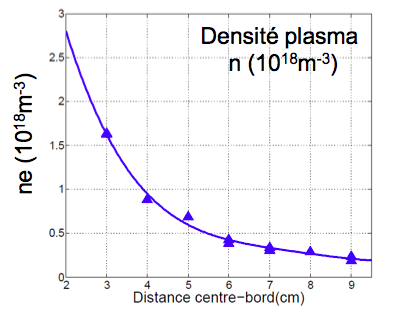
\includegraphics[height=6cm]{figures/4-CybeleExp.png}}
    \subfigure[]{\label{4-CybeleExp2}
    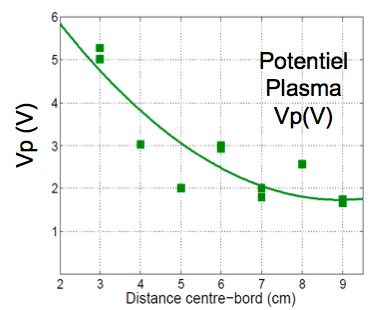
\includegraphics[height=6cm]{figures/4-CybeleExp2.png}}
    \subfigure[]{\label{4-CybeleExp3}
    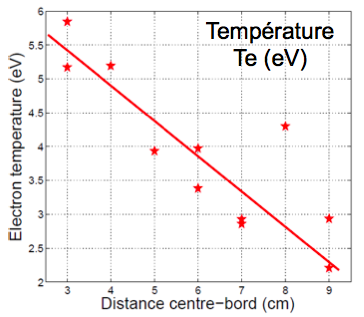
\includegraphics[height=6cm]{figures/4-CybeleExp3.png}}
    \caption{Profils expérimentaux de densité\subref{4-CybeleExp1}~, de
    potentiel\subref{4-CybeleExp2}~ et de
    température\subref{4-CybeleExp3}~ obtenus sur Cybele par
    mesures de sondes~\parencite{SimoninHDR}.}
    \label{4-CybeleExp}
\end{figure}
\begin{figure}[!htbp]
  \centering
    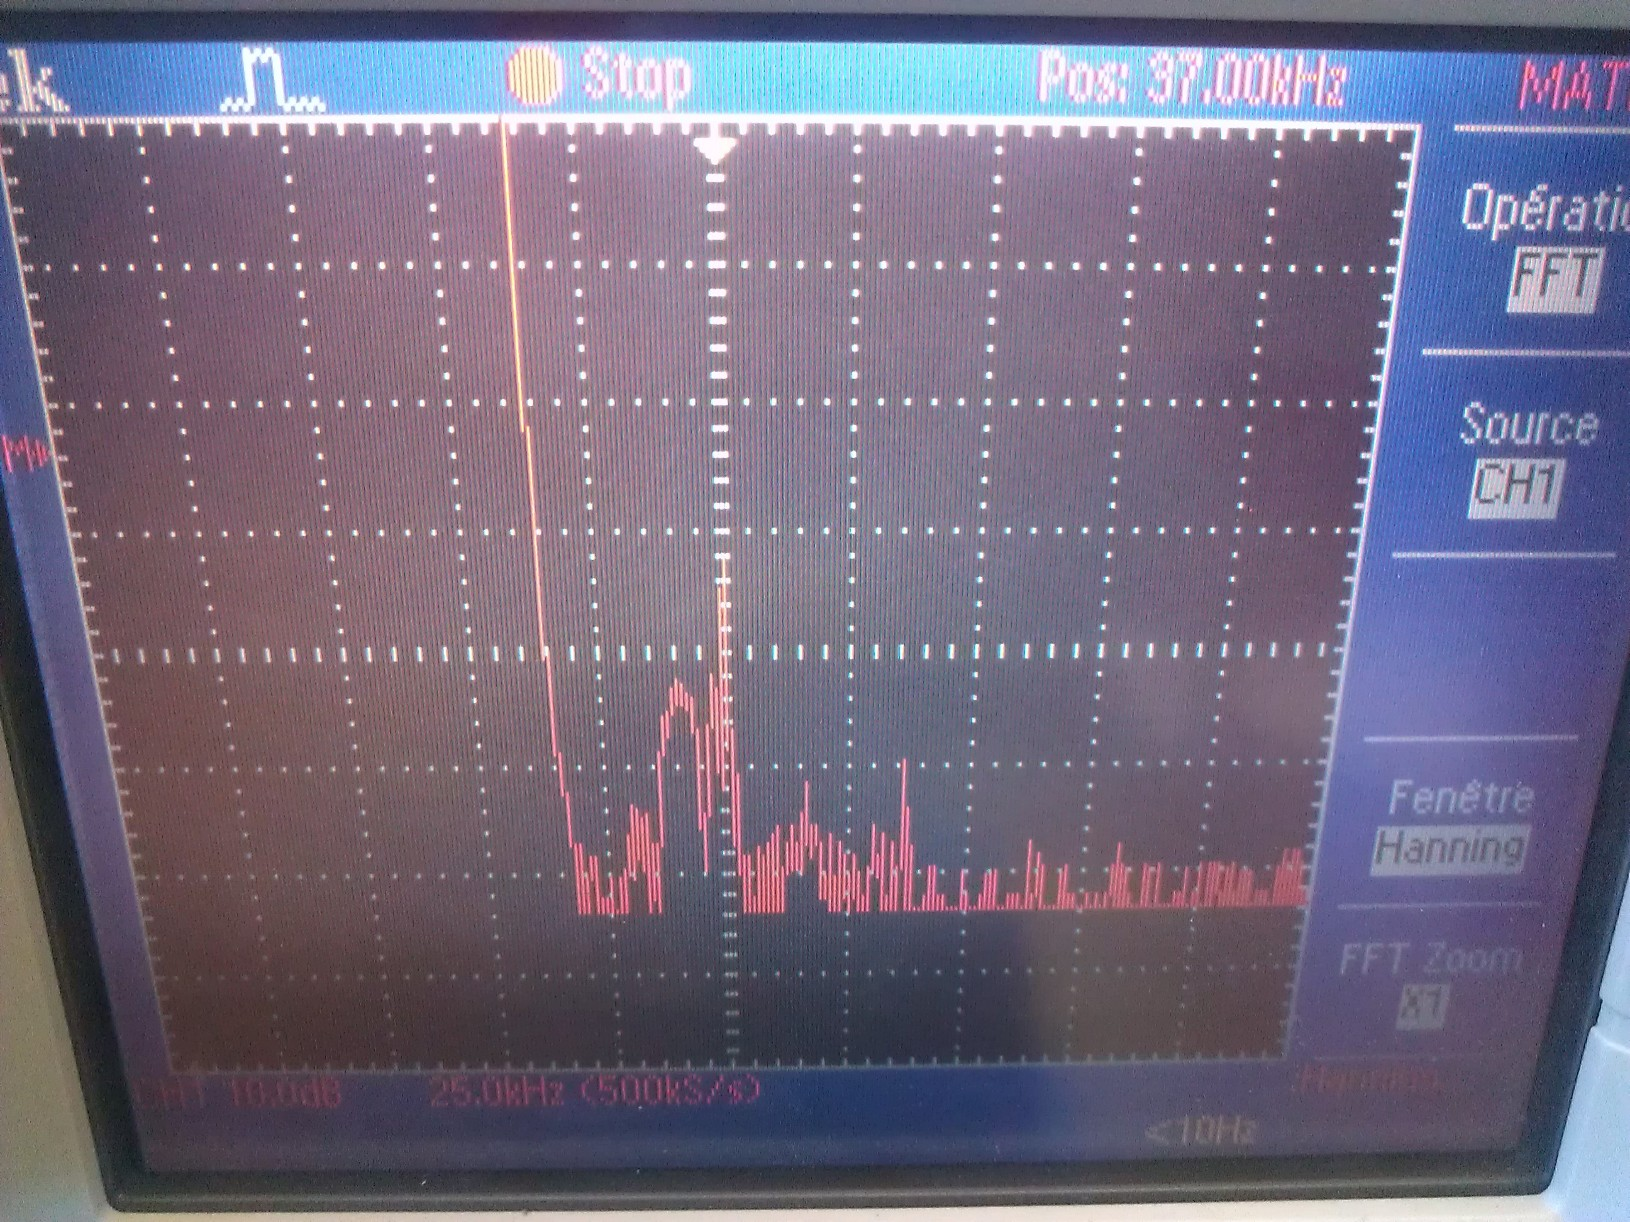
\includegraphics[height=6cm]{figures/4-CybeleFourierSignal.jpg}
    \caption{Spectre du courant de saturation
    ionique à $r\,$= 5 cm du centre de la source.
    L'oscilloscope est réglé sur 25 kHz/carreau.\label{4-CybeleFourierSignal}}
\end{figure}

Dans Cybele, le plasma est chauffé en injectant un courant
d'électron très énergétique à l'aide de filaments. Notre cas de
test, lui, suppose une puissance directement absorbée ; ce n'est évidemment pas
la même chose, mais la physique sous-jacente reste très liée. Une puissance
absorbée est plutôt caractéristique d'un chauffage RF. Cependant, dans une future version de Cybele, il est aussi
prévu d'utiliser une antenne hélicon, qui couplera la puissance par absorption d'énergie.
 
\subsection{Simulation d'une colonne de plasma}

Commençons par montrer les résultats d'une simulation avec des conditions
typiques, dont les paramètres sont donnés dans le tableau~\ref{4-CybeleParam1} :

\begin{table*}[!htbp]
\footnotesize\centering
\ra{1.3}
\begin{tabular}{cc}\toprule
\multicolumn{2}{c}{\bf Paramètres}\\
\midrule 
Parois & Conductrices\\
$L_x$, $L_y$ & 20 cm\\
$L_z$ & 120 cm\\
$B$&100 G, uniforme\\
$\mathcal{P}_\text{ext}$&100 W\\
$l_\mathcal{S}$, $x_\mathcal{S}$& 1 cm, 10 cm\\
$\text{gaz (H}_2\text{)}$ & 1.6 mTorr\\
\bottomrule
\end{tabular}
\caption{Paramètres de la simulation.}\label{4-CybeleParam1}
\end{table*}

 Le domaine de
simulation, illustré sur la figure~\ref{4-cybeleSimDomain}, est de dimension
20~cm~x~20~cm~x~120~cm et représente toujours le plan transverse au champ
magnétique, qui est pris uniforme et d'intensité $B\,$= 100 G. Le plasma est créé au centre du domaine par un chauffage de forme gaussienne en 2D, de largeur $l_\mathcal{S}\,$= 1 cm et en supposant une puissance absorbée
d'environ 100 W.
La pression de gaz (H$_2$) est fixée à 1.6~mTorr avec toutes les parois
conductrices et reliées à la masse (exceptées celles aux extrémités les lignes
de champ qui seront prises de nature isolante dans un cas test).


\begin{figure}[!htbp]
\centering
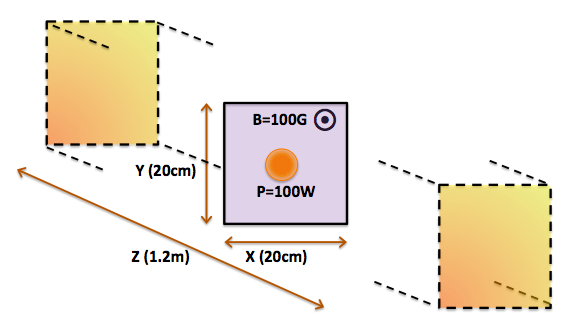
\includegraphics[width=0.8\textwidth]{figures/4-cybeleSimDomain.png}
{\caption{Le domaine de simulation est le plan perpendiculaire au champ
magnétique.}
\label{4-cybeleSimDomain}}
\end{figure}

Les solutions moyennées et instantanées obtenues par MAGNIS avec ces paramètres
sont illustrées sur les figures~\ref{CybeleCartesMoy} et
~\ref{CybeleCartesBase}. La densité est maximale\footnote{La densité maximale du plasma est directement contrôlée par la puissance
absorbée. Bien que celle-ci soit de deux ordres de grandeur inférieure à la
densité mesurée dans Cybele, il suffit de choisir une puissance absorbée
cohérente pour obtenir un résultat proche des mesures expérimentales.} au centre
de la source à 3.10$\puissance{16}$ m$\puissance{-3}$\footnote{La densité
maximale simulée est de deux ordres de grandeur en dessous des valeurs
expérimentales en raison de la puissance absorbée très inférieure (100~W par
rapport à 100~kW dans l'expérience).}, et exponentiellement
décroissante sur une longueur de 2 à 3 cm.
Le potentiel décroît monotonement de 12 V à 0 V dans la direction radiale.
 La température présente quant à elle un fort gradient, passant de 10~eV à moins
 d'1~eV sur 2 à 3~cm de longueur.

\begin{figure}[!htbp]
  \centering
    \subfigure[]{\label{4-CybeleCarteDensiteMoy}
    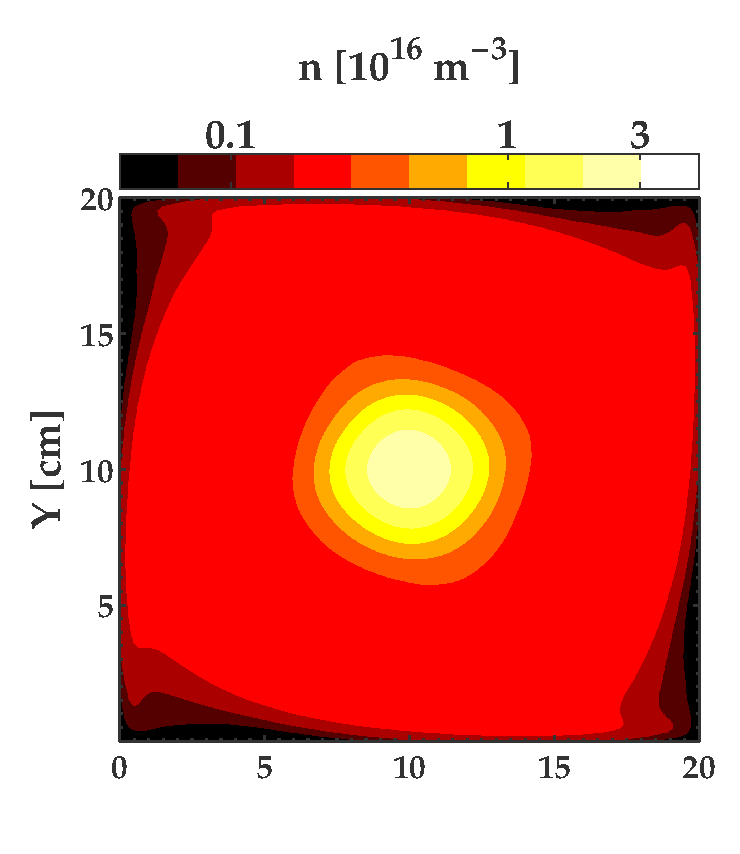
\includegraphics[height=5.5cm]{figures/4-CybeleCarteDensiteMoy.eps}}
    \subfigure[]{\label{4-CybeleCartePotentielMoy}
    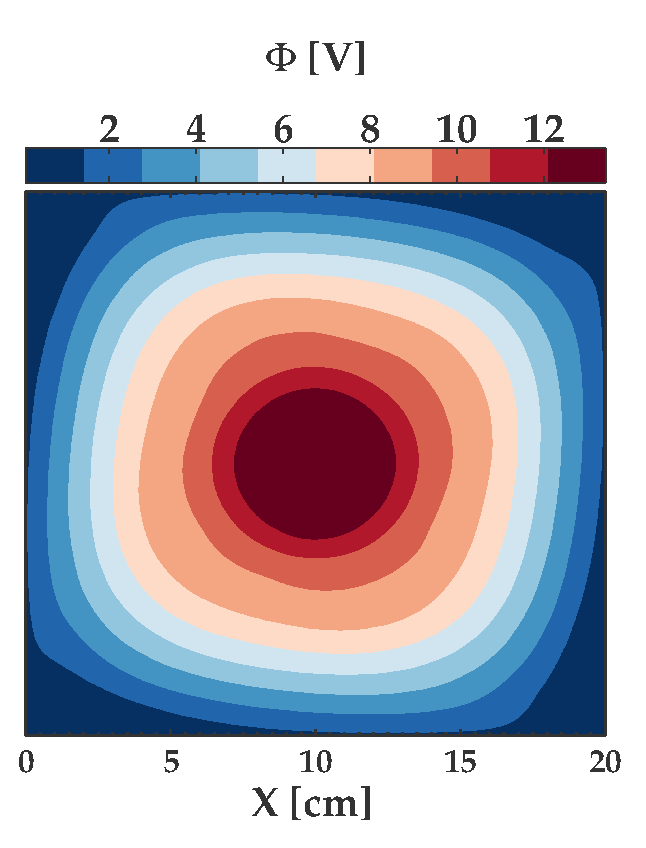
\includegraphics[height=5.5cm]{figures/4-CybeleCartePotentielMoy.eps}}
    \subfigure[]{\label{4-CybeleCarteTemperatureMoy}
    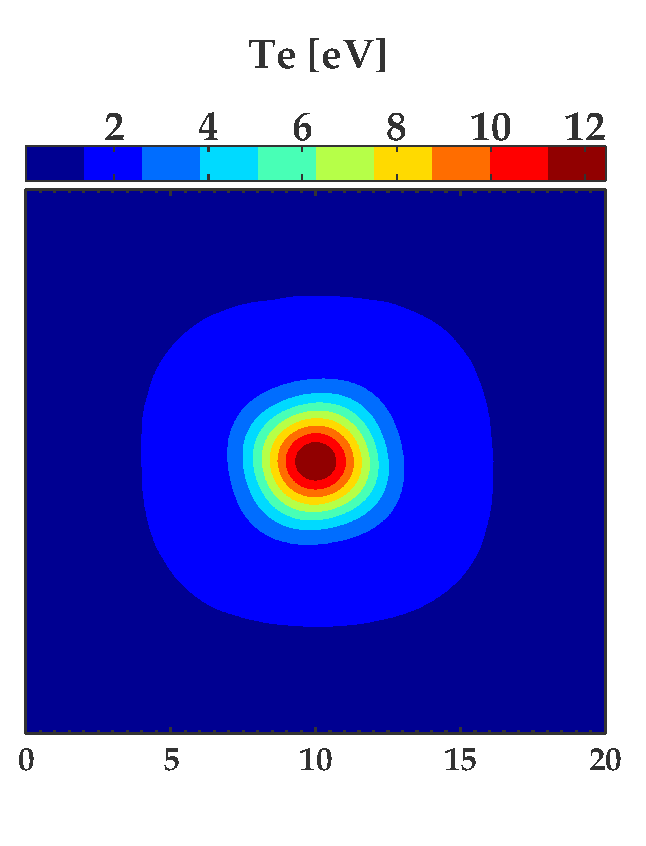
\includegraphics[height=5.5cm]{figures/4-CybeleCarteTemperatureMoy.eps}}
    \caption{Cartes moyennées en temps de
    densité~\subref{4-CybeleCarteDensiteMoy}~, de potentiel~\subref{4-CybeleCartePotentielMoy}~ et de
    température~\subref{4-CybeleCarteTemperatureMoy}.}
    \label{CybeleCartesMoy}
\end{figure}

\begin{figure}[!htbp]
  \centering
    \subfigure[]{\label{4-CybeleCarteDensiteBase}
    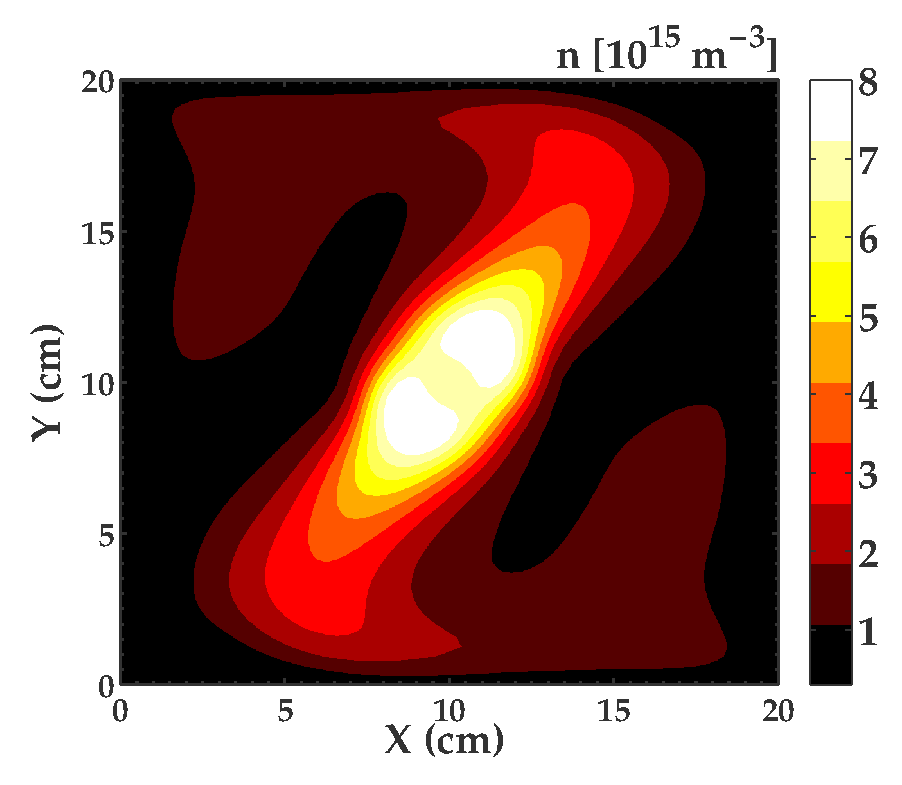
\includegraphics[height=5.5cm]{figures/4-CybeleCarteDensiteBase.eps}}
    \subfigure[]{\label{4-CybeleCartePotentielBase}
    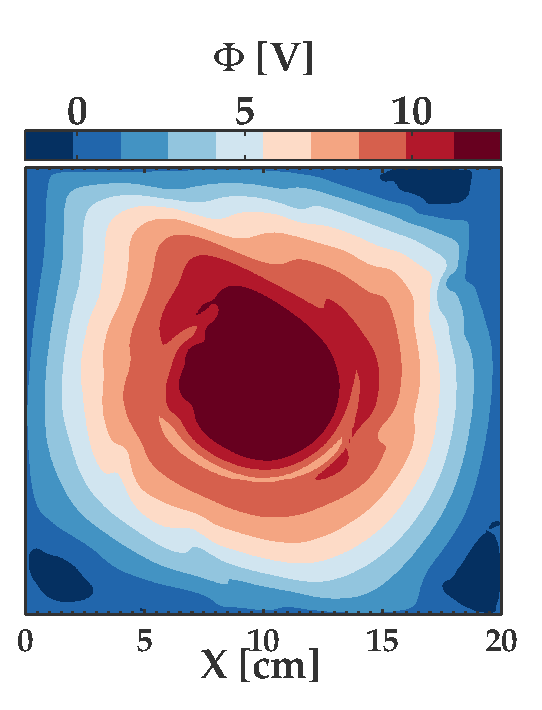
\includegraphics[height=5.5cm]{figures/4-CybeleCartePotentielBase.eps}}
    \subfigure[]{\label{4-CybeleCarteTemperatureBase}
    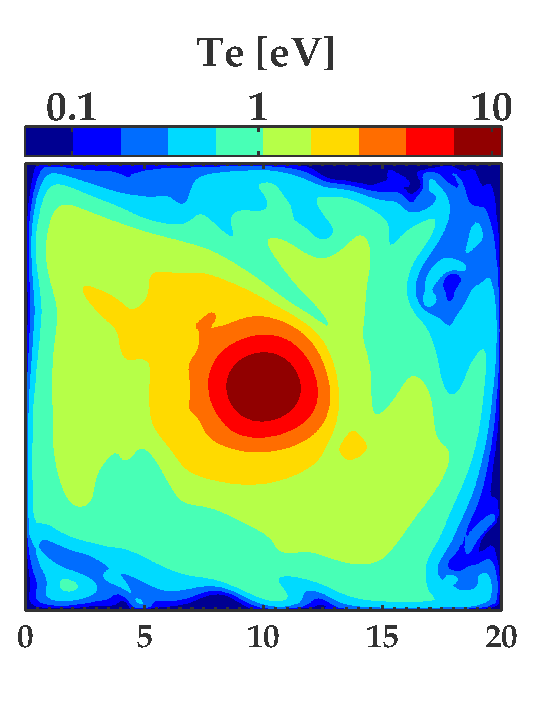
\includegraphics[height=5.5cm]{figures/4-CybeleCarteTemperatureBase.eps}}
    \caption{Cartes instantanées de densité~\subref{4-CybeleCarteDensiteBase}~,
    de potentiel~\subref{4-CybeleCartePotentielBase}~ et de
    température~\subref{4-CybeleCarteTemperatureBase}.}
    \label{CybeleCartesBase}
\end{figure}

 Sur les cartes instantanées 
 (figure~\ref{CybeleCartesBase}), le phénomène le plus remarquable est
 cependant la formation d'un bras de plasma (ou un long filament en 3D) partant
 de la zone centrale et tournant à une vitesse angulaire constante.
Une rotation complète de cette structure de mode $m\,$= 1 s'effectue en
$t\simeq\,$23~\micro s, correspondant à une vitesse angulaire de :

\begin{equation}
\Omega_R=\frac{2\pi}{t}\simeq2.25\;10^5\text{rad/s}
\end{equation}
Les images enregistrées avec des caméras rapides lors des expérimentations
sur les colonnes ont déjà montré un
comportement similaire du plasma (voir figure~\ref{4-CybeleNagdis}). 

\begin{figure}[!htbp]
\centering
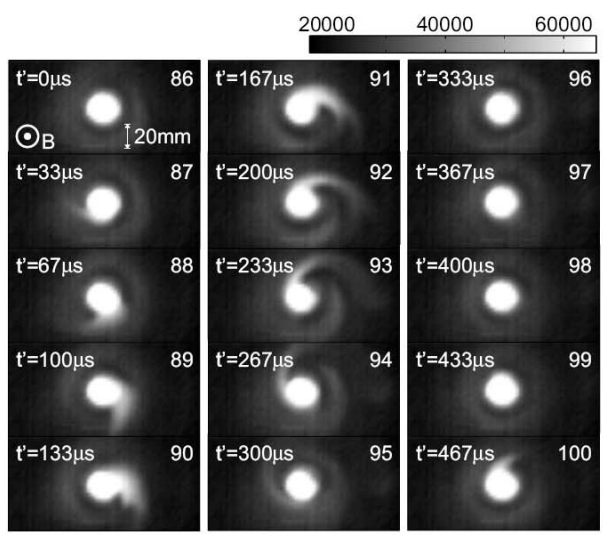
\includegraphics[width=0.5\textwidth]{figures/4-CybeleNAGDIS.png}
\caption{Images successives prises par caméra rapide~\parencite{NagdisCamera}.
La structure effectue une rotation complète en 230 \micro s et apparaît par
intermittence.
\label{4-CybeleNagdis}}
\end{figure}

Dans les colonnes de plasma magnétisées, les électrons ont tendance à s'échapper
le long des lignes de champ dans la direction parallèle. Le courant parallèle,
montré sur la figure~\ref{4-cybeleCartePotentielSurTe}, est déterminé par les
conditions de gaine de Bohm~\parencite{Stangeby} et entièrement gouverné par le
rapport $e\Phi/T_e$. Au centre du plasma, la température électronique est très
élevée. Pour retenir les électrons, le potentiel plasma augmente, atteignant un
ratio $e\Phi/T_e$ de 1.1515. Ce ratio correspond à une densité de courant
parallèle négative de :

\begin{equation}
\mathbf j_\para=enc_s(1-\exp(\Lambda-1.1515))\sim -600\text{A.m}\puissance{-2}
\end{equation}

\begin{figure}[!htbp]
  \centering
    \includegraphics[height=6cm]{figures/4-CartePotentielSurTe.eps}
    \caption{Carte du courant parallèle.
    L'échelle de valeur a été tronquée à
    [-17 17]A/m$^2$ pour une meilleure
    visibilité. Au centre, le courant atteint
    - 700 A/m$^2$.\label{4-cybeleCartePotentielSurTe}}
\end{figure}

En dehors du plasma central, le ratio devient légèrement supérieur
au potentiel flottant, inversant le signe du courant récupéré au bout des lignes
de champ sur une grande partie du domaine. À la frontière entre ces
deux régions (un cercle de rayon $r\sim\,$2,5 cm autour du centre du domaine),
on peut supposer un changement radical de la nature du transport du courant.

\begin{figure}[!htbp]
  \centering
    \subfigure[]{\label{4-CybeleProfilsRadial}
    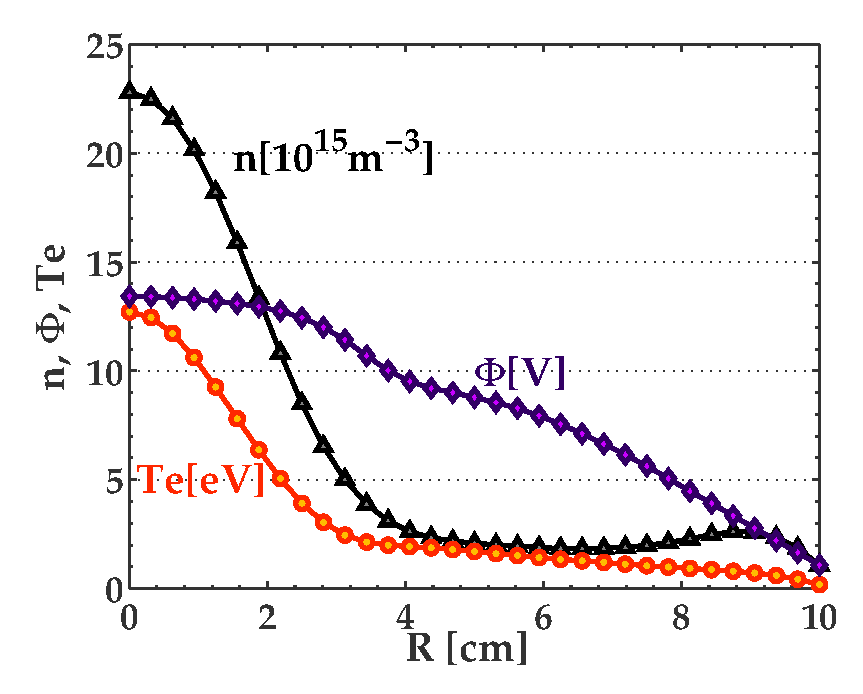
\includegraphics[height=5.2cm]{figures/4-CybeleProfileTempRadiale.eps}}
    \subfigure[]{\label{4-CybeleProfilsAzim}
    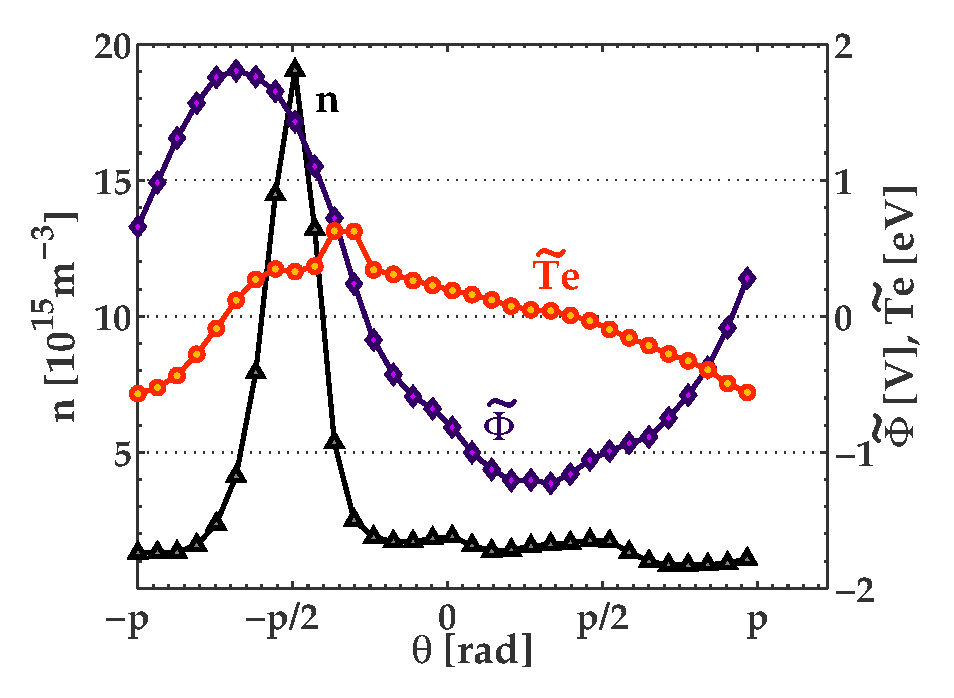
\includegraphics[height=5.2cm]{figures/4-CybeleProfileTempPol.eps}}
    \caption{Profils radiaux~\subref{4-CybeleProfilsRadial}~ et
    azimutaux~\subref{4-CybeleProfilsAzim}~ moyennés en temps de la densité, du
    potentiel et de la température. Le profil radial est pris du centre de la source au bord droit
    en $x\,$= 20 cm. Le profil azimutal est moyenné sur un repère tournant qui
    suit la structure de densité à $r\,$= 5 cm du centre de la source. Les
    quantités $\tilde{\Phi}$ et $\tilde{T}_e$ sont les variations de potentiel et de température par rapport à leur valeur
    moyenne, qui sont respectivement égale à 9 V et 2 eV. La structure se
    déplace dans le sens horaire, i.e. dans la direction des $\theta$ croissants
    sur la figure.}
    \label{4-CybeleProfils}
\end{figure}

La figure~\ref{4-CybeleProfilsRadial} montre le profil radial moyenné dans le
temps des précédents champs, du centre de la source au bord $x\,$= 20 cm. Le
plasma est confiné sur un rayon d'environ 4 cm tandis que le potentiel plasma
diminue progressivement, bien que de façon un peu plus prononcée juste après la
chute de densité du plasma. 
Les profils azimutaux (figure~\ref{4-CybeleProfilsAzim})  sont calculés en
repérant le pic de densité puis en le plaçant en $\theta=-\pi/2$ à chaque pas de temps. Le profil
est ensuite moyenné sur l'ensemble de la durée de la simulation.
On peut remarquer la présence d'une légère avance de phase de la température
sur la densité. Le potentiel, de son côté, est de forme sinusoïdale et montre
aussi un déphasage, dans le sens opposé, avec la densité.

Pour caractériser un peu plus la rotation, intéressons nous
maintenant aux flux électronique et ionique dans la direction
transverse, illustrés sur la figure~\ref{4-CybeleCarteFlux}.
Les ions, créés au centre de la source, traversent le champ magnétiques et
tombent aux parois en effectuant des spirales dans le même sens que le bras de
densité. On constate que le courant ionique est maximal au centre de la source,
et que le flux est plus fort au niveau du bras de densité. La
vitesse du fluide ionique est cependant deux à trois fois moins importante que la vitesse de rotation de
la structure. Sur la seconde image, on peut remarquer que le fluide électronique
change de direction après un minimum, situé là encore aux alentours de la
frontière du plasma confiné.

\begin{figure}[!htbp]
  \centering
    \subfigure[]{\label{4-CybeleCarteFluxIBase}
    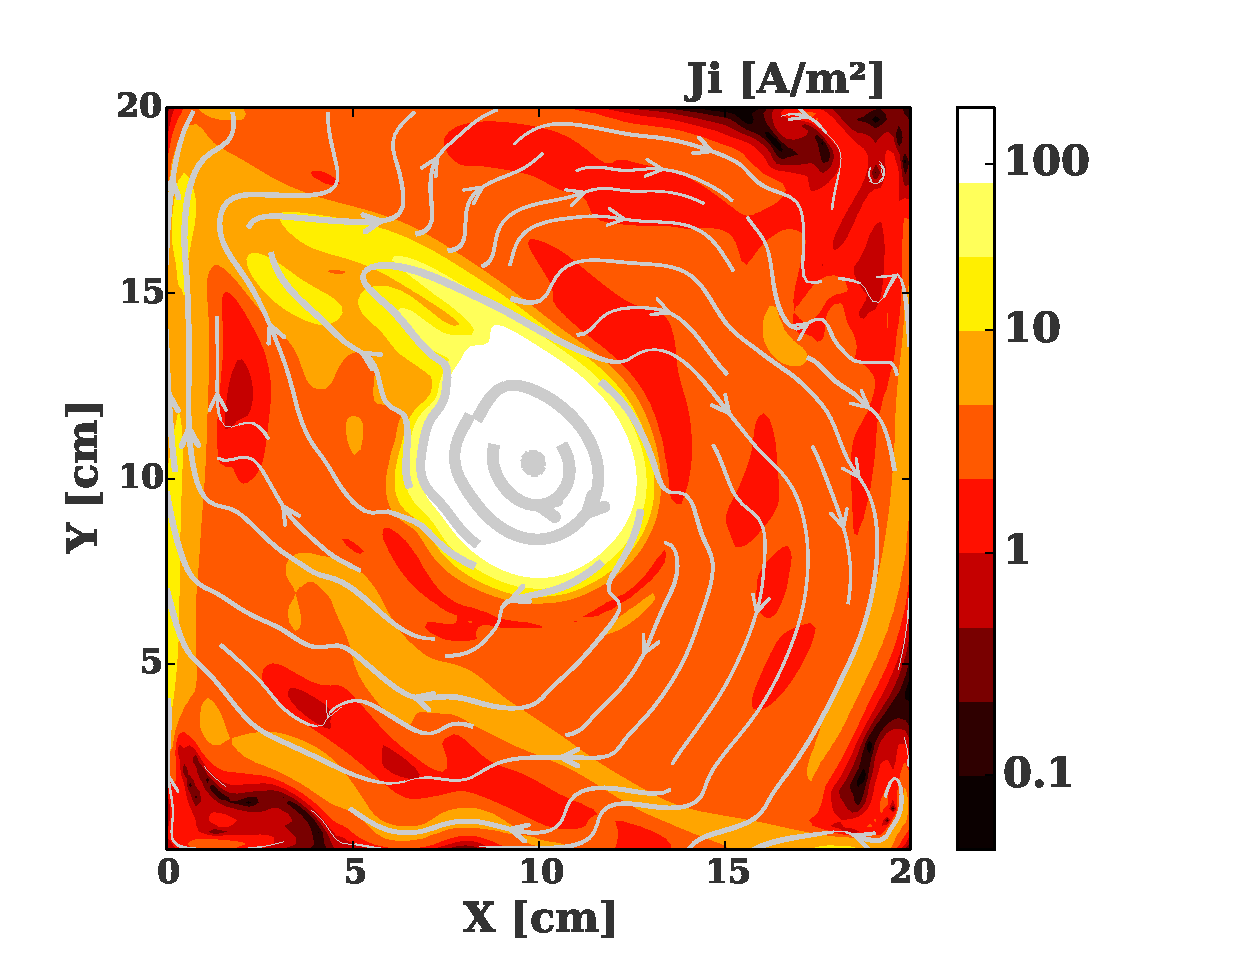
\includegraphics[height=5.5cm]{figures/4-CybeleCarteFluxIBase.eps}}
    \subfigure[]{\label{4-CybeleCarteFluxEBase}
    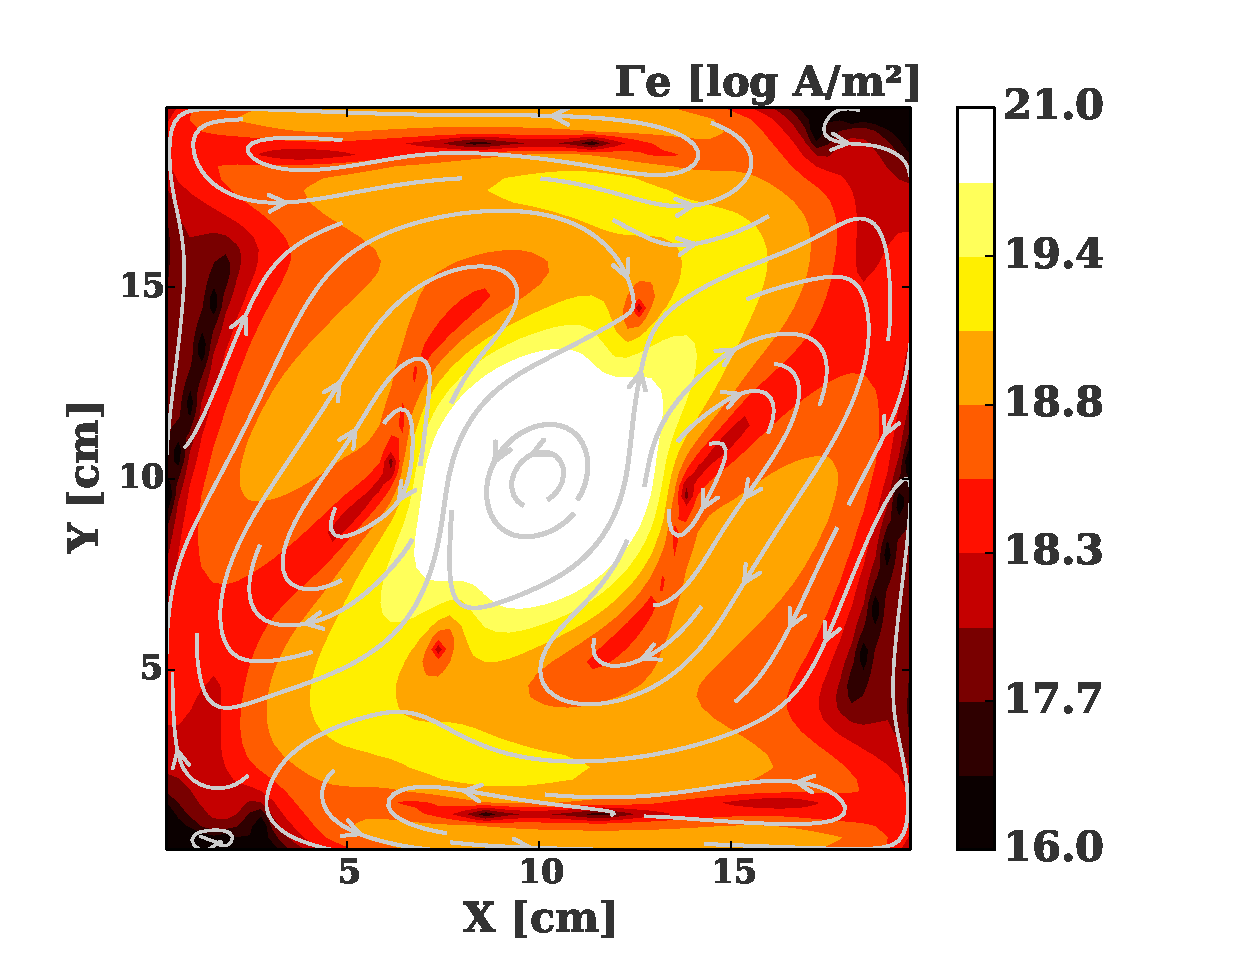
\includegraphics[height=5.5cm]{figures/4-CybeleCarteFluxEBase.eps}}
    \caption{Densités de courant ionique
    \subref{4-CybeleCarteFluxIBase}~ et électronique~\subref{4-CybeleCarteFluxEBase}.}
    \label{4-CybeleCarteFlux}
\end{figure}

Dans la direction radiale et en présence d'un champ magnétique, les gradients
moyens de potentiel et de pression donnent naissance à des dérives
fluides. 
Le champ électrique radial moyen $E_r=-\nabla_r\Phi$ d'environ 120 V/m,
entraîne théoriquement une dérive azimutale de l'ordre de :

\begin{equation}
\Omega_E=\frac{E_r}{rB}\simeq10^5\,\text{rad/s} 
\end{equation}

qui est du même ordre de grandeur que la vitesse de rotation du bras de plasma.
La figure~\ref{4-CybeleVitessesDerive} montre les profils des vitesses
de dérive électrique et diamagnétique le long de la direction radiale. On
observe que la vitesse de dérive diamagnétique, i.e. liée au gradient de
pression, est dominante au centre du plasma. 

\begin{figure}[!htbp]
\centering
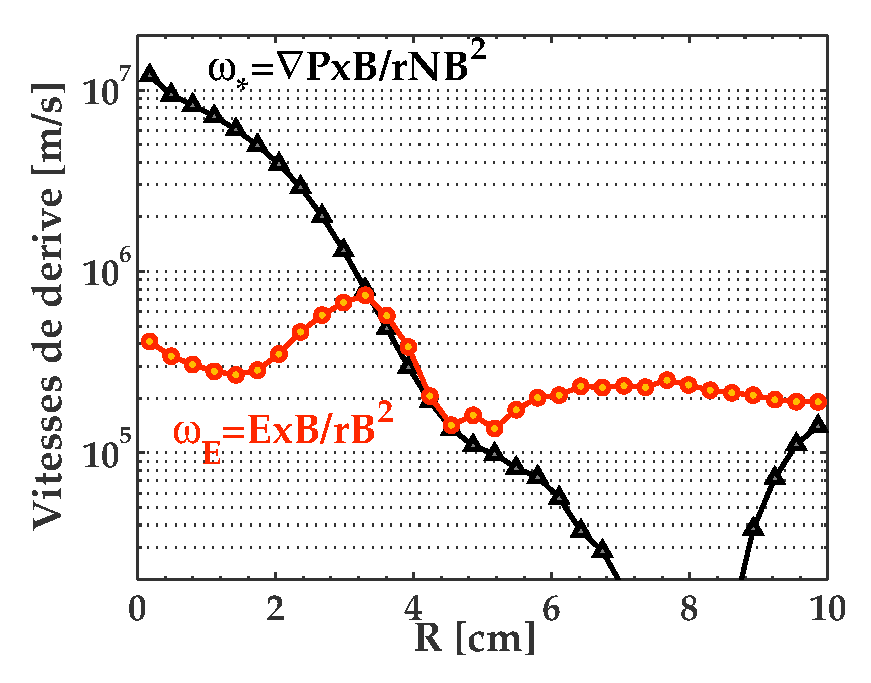
\includegraphics[width=0.5\textwidth]{figures/4-CybeleProfileVitessesDerive.eps}
{\caption{Carte de densité à 35G.}
\label{4-CybeleVitessesDerive}}
\end{figure}

Cette dérive entraîne les ions et les électrons dans des directions
contraires, générant un fort courant. À $r\sim\,$4~cm, au niveau de la
séparation, les deux vitesses s'égalisent, puis la vitesse de dérive électrique, qui ne
génère que peu de courant, prend le dessus. Dans la région traversée par le bras
de densité, $\Omega_E\simeq$ 2,3.10$\puissance{5}\,\text{rad.s}\puissance{-1}$
est très proche de la vitesse de rotation mesurée.

Lors de l'exploration des modes de fonctionnement de la source, le transport
dans la colonne de plasma s'est révélé principalement sensible à deux
paramètres : l'intensité du champ magnétique et les conditions parallèles 
(longueur de la source et nature des parois). Les deux sections suivantes
montrent un rapide aperçu de l'influence de ces deux variables.

\subsection{Variation croissante du champ magnétique}
Nous reprenons dans cette partie les conditions de base utilisées précédemment,
en faisant varier l'intensité du champ magnétique de 0 G à 170 G (cf.
tableau~\ref{4-CybeleBParam})

\begin{minipage}{\textwidth}
\footnotesize\centering
\ra{1.3}
\begin{tabular}{lcclc}\toprule
\multicolumn{5}{c}{\bf Paramètres}\\
\midrule 
Parois & Conductrices &&$L_x$, $L_y$, $L_z$  & 20cm, 20cm,
120cm\\
$\mathcal{P}_\text{ext}$&100W&&$l_\mathcal{S}$, $x_\mathcal{S}$&1cm, 10cm\\
$\mathbf B$ &\textbf{1--170 G, uniforme}&&$\Delta t$, $\Delta x$&10$^{-8}$s,
0.15cm\\
gaz (H_2) & 1.6 mTorr&&&\\
\bottomrule
\end{tabular}
\captionof{table}{Paramètres de la simulation.}\label{4-CybeleBParam}
\end{minipage}	

En l'absence de champ magnétique, le transport est isotrope. Le plasma
d'hydrogène a une densité de 3.10$\puissance{14}$~m$\puissance{-3}$ et sa
température, assez homogène, est de 11~eV. Ajoutons maintenant un champ
magnétique ; au fur et à mesure de la montée en intensité du champ, on peut
repérer quatre modes de fonctionnement.

\begin{figure}[!htb]
  \centering
    \subfigure[]{\label{4-CybeleVarMag1}
    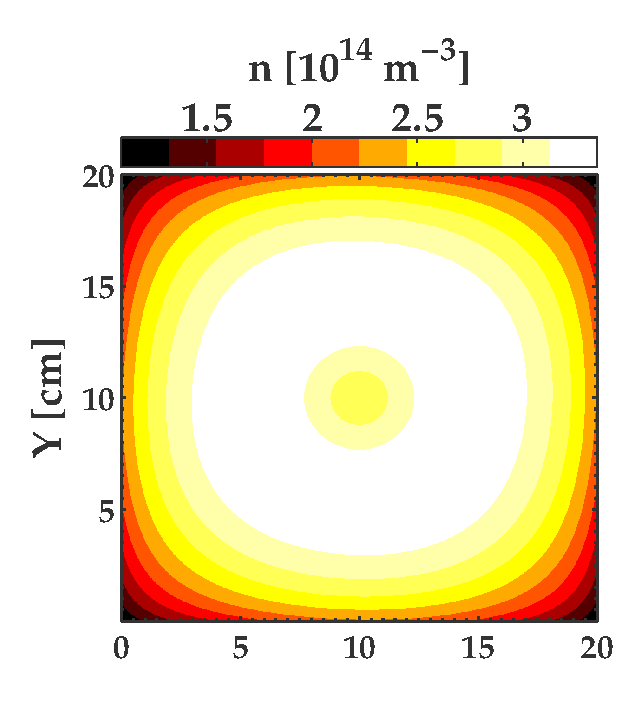
\includegraphics[height=5.5cm]{figures/4-CybeleVarMag1.eps}}
    \subfigure[]{\label{4-CybeleVarMag2}
    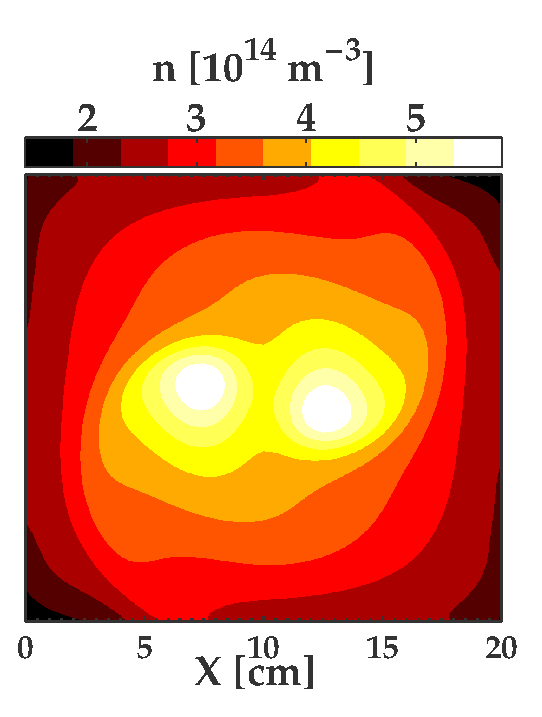
\includegraphics[height=5.5cm]{figures/4-CybeleVarMag2.eps}}
    \subfigure[]{\label{4-CybeleVarMag3}
    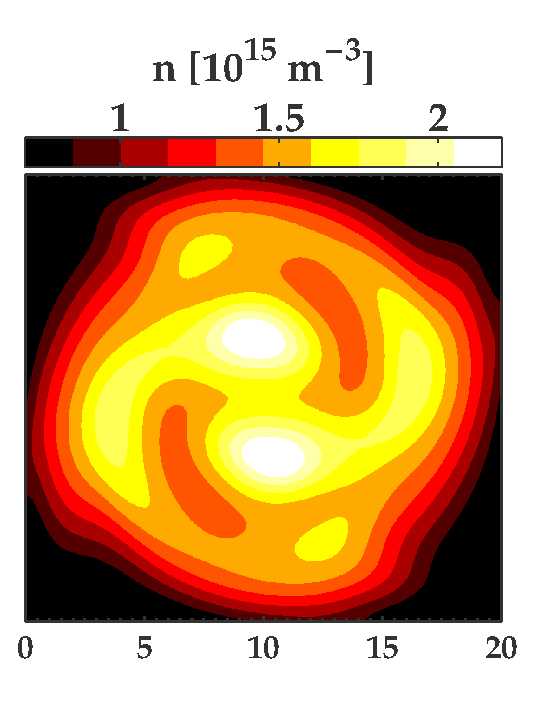
\includegraphics[height=5.5cm]{figures/4-CybeleVarMag3.eps}}
    \caption{Cartes de densité à 1 G~\subref{4-CybeleVarMag1}~, 4
    G~\subref{4-CybeleVarMag2}~ et 15 G~\subref{4-CybeleVarMag3}.}
    \label{4-CybeleVarMag-1}
\end{figure}

\subsubsection{de 1G à 2G}

L'application d'un faible champ magnétique modifie légèrement la nature du
transport. Observons la figure~\ref{4-CybeleVarMag1} : entre 1~G et 2~G, le
plasma forme un anneau, de densité équivalente au cas non
magnétisé. La température au centre de la source s'élève, passant 
successivement à 14~eV puis à 20~eV. Le rayon de l'anneau est approximativement
égal au rayon de Larmor électronique local, qui peut être encadré par :
\begin{equation}
\frac{L_\perp}{2}=10\,\text{cm}>\rho\indice{Le}>l_c\simeq 5\,\text{cm}
\end{equation}
où $L_\perp$ est la longueur caractéristique de la source et $l_c$ une longueur
critique déterminant ce régime de fonctionnement. 

\subsubsection{de 3G à 15G}
À partir de 3~G, le plasma perd sa symétrie axiale. Deux îlots de densité plus
élevée apparaissent, tournant à une vitesse angulaire $\Omega_R$ qui varie de 1
à 2.10$\puissance{6}\,\text{rad.s}\puissance{-1}$ sur une orbite de rayon
approximativement égale au rayon de Larmor électronique, qui devient inférieur
à $l_c\,$=~5~cm. La température maximale commence à osciller\footnote{À B=7.5G,
la fréquence cyclotronique électronique est égale à
1,3.10$\puissance{8}\,\text{s}\puissance{-1}$, très proche de la fréquence de
collision des électrons. Le maximum de température atteint son plus haut taux
de fluctuation.} et augmente modérément.

Ce type de fonctionnement, qui est caractérisé par une
fréquence de rotation assez rapide et la présence d'une structure de densité de
mode m = 2, se manifeste jusqu'à un champ magnétique d'une petite vingtaine de
gauss. 


\subsubsection{de 18G à 70G}
Entre 18~G et 30~G, le plasma devient extrêmement instable, comme illustré
sur la figure~\ref{4-CybeleVarMag-2} : le plasma croît en
densité et en température jusqu'à atteindre une valeur critique, puis relaxe
très rapidement en dégageant une bouffée de plasma. La fréquence de ce cycle
est d'environ 5~kHz.

\begin{figure}[htb]
  \centering
    \subfigure[]{\label{4-CybeleVarMag4}
    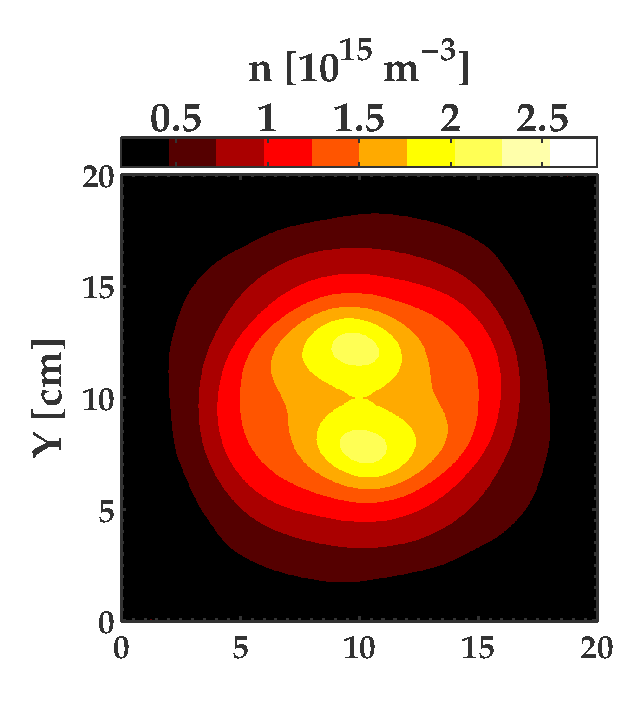
\includegraphics[height=5.5cm]{figures/4-CybeleVarMag4.eps}}
    \subfigure[]{\label{4-CybeleVarMag5}
    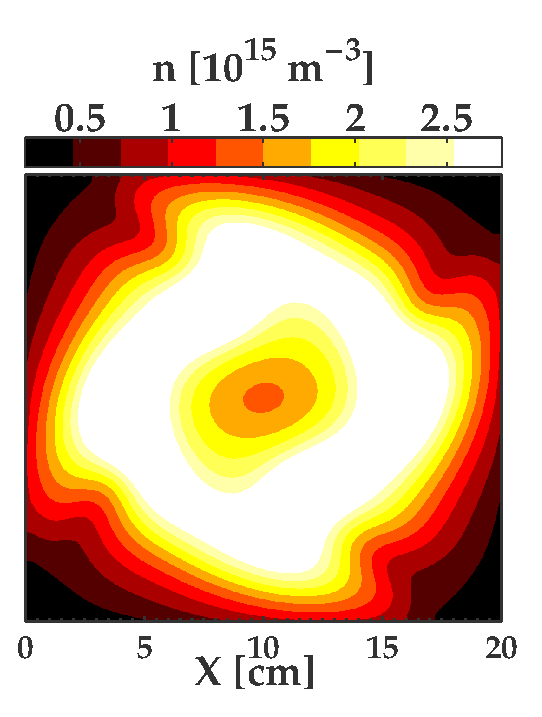
\includegraphics[height=5.5cm]{figures/4-CybeleVarMag5.eps}}
    \subfigure[]{\label{4-CybeleVarMag6}
    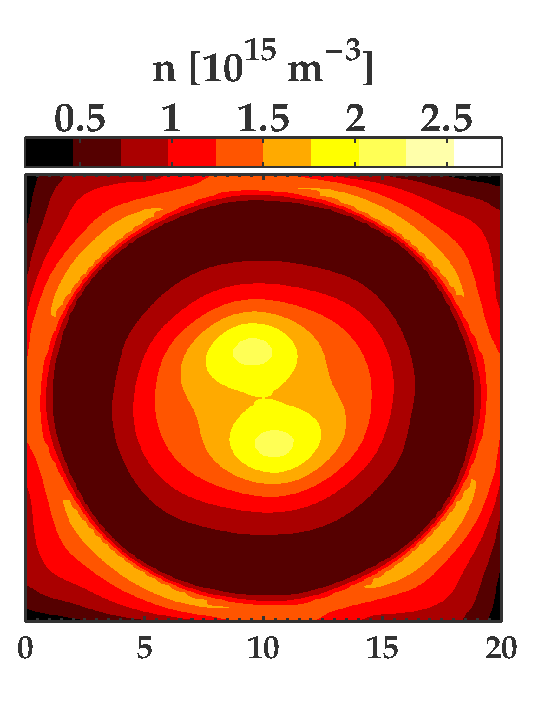
\includegraphics[height=5.5cm]{figures/4-CybeleVarMag6.eps}}
    \caption{Cartes de densité à 20 G à trois instants
    différents ($t\,$=~0$\micro$s,
    $t\,$=~80$\micro$s et $t\,$=~120$\micro$s). Un cycle dure approximativement
    180~$\micro$s.}
    \label{4-CybeleVarMag-2}
\end{figure}

La figure~\ref{4-CybeleVarMag8} montre la forme du plasma à 35~G, qui s'est
stabilisé\footnote{La température moyenne des électrons redescend à une
quinzaine d'électronvolts. Le rayon de Larmor ionique local, qui était
auparavant supérieur à la longueur caractéristique du système, diminue
jusqu'à une longueur de l'ordre de la dizaine de centimètres. Nous supposons
que la "stabilité" du plasma est ici fortement dépendante du ratio entre le
rayon de Larmor ionique et la taille du plasma.}. Plusieurs pics, situés à la
frontière du plasma, sont de densités 2 à 3 fois supérieure à la densité
centrale. On commence aussi à voir apparaître un bras en périphérie du plasma,
qui tourne à une fréquence de 50~kHz.
\begin{figure}[!htb]
\centering
\includegraphics[width=0.33\textwidth]{figures/4-CybeleVarMag8.eps}
{\caption{Carte de densité à 35 G.}
\label{4-CybeleVarMag8}}
\end{figure}

De 35~G à 70~G, le plasma est dans un régime transitoire : la température
oscille fortement, et la densité centrale se relaxe régulièrement à travers 
le mode azimutal, qui se développe de plus en plus.

\subsubsection{de 70G à 170G}
À partir de 70~G, le rayon de Larmor ionique devient inférieur à 5 cm : les ions
peuvent être considérés comme magnétisés.
Sur la figure~\ref{4-CybeleVarMag9}, on voit que le
plasma forme une spirale. La structure azimutale de mode m=1 tourne à une
vitesse de 4.10$\puissance{5}\,\text{rad.s}\puissance{-1}$. Les
figures~\ref{4-CybeleVarMag10} et~\ref{4-CybeleVarMag11} représentent la densité
du plasma à 130~G (où le plasma se déplace en effectuant une rotation presque
solide) et 170~G. Elles se caractérisent par l'apparition d'un mode azimutal
m = 2.
\begin{figure}[!htbp]
  \centering
    \subfigure[]{\label{4-CybeleVarMag9}
    \includegraphics[height=5.5cm]{figures/4-CybeleVarMag9.eps}}
    \subfigure[]{\label{4-CybeleVarMag10}
    \includegraphics[height=5.5cm]{figures/4-CybeleVarMag10.eps}}
    \subfigure[]{\label{4-CybeleVarMag11}
    \includegraphics[height=5.5cm]{figures/4-CybeleVarMag11.eps}}
    \caption{Cartes de densité à 80 G~\subref{4-CybeleVarMag9}~, 130 G
    \subref{4-CybeleVarMag10}~ et 170 G \subref{4-CybeleVarMag11}.}
    \label{4-CybeleVarMag-3}
\end{figure}

Le tableau~\ref{4-CybeleVarMagTab} résume les propriétés du plasma observées
dans cette partie.


\begin{table*}[!htbp]
\footnotesize\centering
\ra{1.3}
\begin{tabular}{@{}ccccccccc@{}}\toprule
B&&\multicolumn{2}{c}{Champs}&&\multicolumn{2}{c}{Échelles} &&
Rotation\\
\cmidrule{3-4} \cmidrule{6-7} \cmidrule{9-9}
&& $n$ (m\textsuperscript{-3}) & $T_e$ (eV)&& $\omega_{c\alpha}$
&$\rho\indice{L\alpha}$&& $\Omega_R$ (10\textsuperscript{5}rad/s)\\
\midrule Phase 1&&&&&\multicolumn{2}{c}{électrons}\\
\scriptsize 1-2 &&\scriptsize 3.3 10\textsuperscript{14} $\nearrow$~~
\scriptsize 3.5 10\textsuperscript{14} &\scriptsize14 $\nearrow$~~\scriptsize 20 &&
$\omega_{ce}<\nu_e$ &\scriptsize$\rho\indice{Le}\sim L_\perp$ && \scriptsize -
\\
Phase 2\\
\scriptsize 3-15 &&\scriptsize 5.5 10\textsuperscript{14}
$\nearrow$~~\scriptsize 1.8 10\textsuperscript{15} &\scriptsize22
$\nearrow$~~\scriptsize 28.5 && $\omega_{ce}\sim\nu_e$
&\scriptsize$\rho\indice{Le}< L_\perp$ && \scriptsize 10 $\nearrow$~~\scriptsize20
\\
Phase 3 &&&&&\multicolumn{2}{c}{ions}\\
\scriptsize 17-60 &&\scriptsize 2 10\textsuperscript{15} $\nearrow$~~\scriptsize
2 10\textsuperscript{16} &\scriptsize$\in$ \scriptsize [26 - \scriptsize 37]
&& $\omega_{ci}<\nu_i$ &\scriptsize$\rho\indice{Li}\sim L_\perp$ && \scriptsize
N.A.
\\
Phase 4 \\
\scriptsize 70-170 &&\scriptsize 1.3 10\textsuperscript{16}
$\nearrow$~~\scriptsize 4.5 10\textsuperscript{16} &\scriptsize23
$\searrow$~~\scriptsize 9 && $\omega_{ci}\sim\nu_i$
&\scriptsize$\rho\indice{Li}< L_\perp$ && \scriptsize 4 $\searrow$~~\scriptsize1.5$\nearrow$~~\scriptsize2
\\
\bottomrule
\end{tabular}
\caption{Tableau résumant les principales
caractéristiques de la colonne de plasma dans un champ
magnétique variant de 1G à 170G.}\label{4-CybeleVarMagTab}
\end{table*}

Pour résumer, on constate qu'à puissance fixée, la densité augmente en
fonction du champ magnétique tandis que la température électronique progresse tout
d'abord jusqu'à une trentaine d'électronvolts, puis redescend sous la barre des
10 eV.
Un mode azimutal se développe avec l'augmentation du champ magnétique, avec un
unique bras tournant à une vitesse angulaire $\Omega_R\sim$ 2.3 10\textsuperscript{5} rad/s. Dans
certaines conditions un deuxième bras peut aussi apparaître. Ce deuxième bras ne
se déplace pas forcément à la même vitesse que le premier. À vitesse égale
les deux bras tournent en phase de part et d'autre du centre de la source, mais
quand l'une des vitesses est inférieure, les bras peuvent se dépasser (et
éventuellement fusionner).

Cette étude sur la variation croissante du champ magnétique montre 
que le plasma peut se comporter très différemment en fonction de
l'intensité du champ, avec parfois la superposition de plusieurs modes de
fonctionnement.

\subsection{Rôle de la direction parallèle}
\begin{minipage}{\textwidth}
\footnotesize\centering
\ra{1.3}
\begin{tabular}{lcclc}\toprule
\multicolumn{5}{c}{\bf Paramètres}\\
\midrule 
Parois & Conductrices / Isolantes &&$L_x$, $L_y$  & 20cm, 20cm\\
\textbf{L}$_z$& \textbf{1--20 m}&&$l_\mathcal{S}$, $x_\mathcal{S}$&1cm, 10cm\\
$\mathcal{P}_\text{ext}$&100W&&$\Delta t$, $\Delta x$&10$^{-8}$s,
0.15cm\\
$B$ & 100 G, uniforme&&&\\
gaz (H_2) & 1.6 mTorr&&&\\
\bottomrule
\end{tabular}
\captionof{table}{Paramètres de la simulation.}\label{4-CybeleZParam}
\end{minipage}	

La direction parallèle joue aussi un rôle très influent dans la
dynamique du plasma. En laissant plus ou moins la possibilité aux électrons (et
donc au courant) de sortir du système par les parois, les contraintes imposées
au transport transverse évoluent. Pour étudier ce paramètre, nous faisons
varier la hauteur de la source (les paramètres sont rappelés sur le
tableau~\ref{4-CybeleZParam}). La figure~\ref{4-CybeleProfileZ} montre les
profils radiaux de densité et de température pour différentes longueurs de source ainsi qu'un cas dans lequel les parois aux extrémités des lignes de champ sont choisies isolantes, et où la conservation du courant ne se joue que dans la
direction perpendiculaire :

\begin{equation}
n_iW_{i_\para}=n_eW_{e_\para}\Leftrightarrow\nabla_\para\cdot\mathbf j_\para = 0
\Rightarrow \nabla_\perp\cdot\mathbf j_\perp = 0
\end{equation}

\begin{figure}[!htbp]
  \centering
    \subfigure[]{\label{4-CybeleProfileDenRadialeZ}
    \includegraphics[height=5.25cm]{figures/4-CybeleProfileDenRadialeZ.eps}}
    \subfigure[]{\label{4-CybeleProfileTempRadialeZ}
    \includegraphics[height=5cm]{figures/4-CybeleProfileTempRadialeZ.eps}}
    \caption{Comparaison des profils de
    densité~\subref{4-CybeleProfileDenRadialeZ}~ et de
    température~\subref{4-CybeleProfileTempRadialeZ}~ pour différentes
    longueurs parallèles}
    \label{4-CybeleProfileZ}
\end{figure}

En toute généralité, on peut constater que l'effet
principal de l'augmentation de la longueur parallèle est de faire monter la
densité tout en abaissant la température électronique.
L'allongement de la source a le même effet que l'augmentation de l'intensité du
champ magnétique, i.e. à certaines longueurs, on voit apparaître sur la densité
une structure azimutale de mode m = 1, voir m = 2.

La figure~\ref{CybeleCartesIsolant} montre les différents champs dans le cas de
parois isolantes. Le plasma, qui ne peut plus s'échapper le long de la direction
parallèle, s'étire dans la direction transverse tandis que la rotation se
saccade.
Le champ électrique et la température dans le plasma sont très faibles, et on
peut observer un anneau s'étalant sur toute la largeur de la source où le
potentiel est un peu plus bas.

\begin{figure}[!htbp]
  \centering
    \subfigure[]{\label{4-CybeleCarteDensiteIsolant}
    \includegraphics[height=5.5cm]{figures/4-CybeleCarteDensiteIsolant.eps}}
    \subfigure[]{\label{4-CybeleCartePotentielIsolant}
    \includegraphics[height=5.5cm]{figures/4-CybeleCartePotentielIsolant.eps}}
    \subfigure[]{\label{4-CybeleCarteTemperatureIsolant}
    \includegraphics[height=5.5cm]{figures/4-CybeleCarteTemperatureIsolant.eps}}
    \caption{Cartes de densité \subref{4-CybeleCarteDensiteIsolant}~, de
    potentiel \subref{4-CybeleCartePotentielIsolant}~ et de
    température \subref{4-CybeleCarteTemperatureIsolant}~ dans le cas de parois
    diélectriques au bout des lignes de champ.}
    \label{CybeleCartesIsolant}
\end{figure}		

Dans cette partie, nous avons tout d'abord vu que 
les solutions calculées par MAGNIS pour une colonne de plasma
sont plutôt cohérentes : qualitativement, le plasma est confiné dans le plan
transverse et en rotation. La forme caractéristique en spirale, ainsi que
l'instationnarité du plasma observées en manipulation sont reproduites. 
Enfin, nous avons montré que la direction parallèle joue un rôle crucial dans
les mécanismes du transport magnétisé, et qu'il est donc nécessaire de
tenir compte des pertes en particules et en courant le long du champ magnétique
pour bien capter la physique sous-jacente.

\section{Plasma de bord de tokamaks}

Cette dernière partie est consacrée à la configuration hautement magnétisée
de la SOL, qui correspond à un cas limite de notre étude. Le premier objectif
est toujours de vérifier la validité des solutions calculées par MAGNIS ; 
nous les comparons pour cela avec les résultats de
TOKAM dans sa version isotherme avec conditions aux limites dans la direction
radiale.

\subsection{Un cas critique pour MAGNIS}
Les modèles décrivant les plasmas de SOL ont tous un
point commun :
ils sont construits avec une hypothèse d'ordering basée sur la forte magnétisation des
particules, ce qui permet de simplifier considérablement les équations
du transport transverse dans le plasma, en séparant le mouvement cyclotronique
des mouvements de dérive.
Cette hypothèse d'ordering n'est
toutefois pas faite dans MAGNIS, l'objectif étant de pouvoir simuler à la
fois les plasmas faiblement et fortement magnétisés. 

La simulation d'un plasma de type SOL avec MAGNIS constitue ainsi un cas idéal
pour :

\begin{itemize}
  \item valider les solutions du transport magnétisé calculées par MAGNIS
  \item	tester le schéma numérique du modèle, dans le cadre d'un plasma
  totalement ionisé et turbulent
 \end{itemize}
  
\begin{figure}[!htbp]
\centering
\includegraphics[width=0.5\textwidth]{figures/4-tokamSimDomain.png}
\caption{Le domaine de simulation est identique à celui présenté au
chapitre II. La boîte correspond à une petite région de la SOL, de dimension
2cm x 2cm, simulant le côté HFS à gauche de la source et le côté LFS à droite.
\label{4-tokamSimDomain}}
\end{figure}

\begin{table*}[!htbp]
\footnotesize\centering
\ra{1.3}
\begin{tabular}{lcclc}\toprule
\multicolumn{5}{c}{\bf Paramètres}\\
\midrule 
Parois & Conductrices&&$L_x$, $L_y$, $L_z$  & 2 cm, 2cm, 10 m\\
$B$&1 T&& légèrement décroissant&\\
$T_e$&1 eV&& plasma isotherme& \\
$\mathcal{P}_\text{ext}$&1 kW&&$l_\mathcal{S}$, $x_\mathcal{S}$& 0.2 mm, 0.6
cm\\
$\text{gaz (H}_2\text{)}$ & -- &&$\Delta t$, $\Delta x$&10$^{-8}$s, 10$^{-4}$m\\
\bottomrule
\end{tabular}
\caption{Paramètres de la simulation.}\label{4-CybeleParam3}
\end{table*}

Nous reprenons les paramètres et la géométrie de simulation utilisés dans le
chapitre~\ref{chapitre3}. Le champ magnétique, à peu près égal à 1~T, est
choisi linéairement décroissant jusqu'à 0.98~T sur le bord droit du
domaine\footnote{Ce choix correspond à un coefficient de courbure des lignes de
champ g~=~5.10$^{-4}$ (cf.~\S~\ref{chapitre3}-\ref{2-flute})}.
Le plasma est considéré isotherme et la densité de neutre est égale à zéro. La
taille de la zone simulée, dont on rappelle la géométrie
figure~\ref{4-tokamSimDomain}, est de 2~cm~x~2~cm soit à peu près
200~$\rho_{Li}$ pour une température électronique de 1 eV. La longueur de la boîte dans la direction du champ magnétique est choisie égale à 10 m pour obtenir une
conductivité parallèle $\sigma$~=~10$^{-5}$. Ces paramètres de simulation sont
rappelés dans le tableau~\ref{4-CybeleParam3}.

\begin{figure}[!htbp]
  \centering
    \subfigure[]{\label{4-Tokam1}
    \includegraphics[height=8cm]{figures/4-Tokam1.eps}}
    \subfigure[]{\label{4-Tokam2}
    \includegraphics[height=8cm]{figures/4-Tokam2.eps}}
    \caption{Carte de densité telle que calculée par MAGNIS~\subref{4-Tokam1}~
et par TOKAM~\subref{4-Tokam2}. La densité calculée par TOKAM est ici
redimensionnée avec $n_0~\simeq$~10$^{19}$~m$^{-3}$.}
    \label{4-TokamDensite}
\end{figure}


La figure~\ref{4-TokamDensite} présente les cartes de densité
calculées par MAGNIS et par TOKAM pour ces conditions. On peut
constater que MAGNIS donne des résultats remarquablement proches de ceux
escomptés au vu de la différence de conception entre les deux modèles. 

Tout d'abord, il arrive à capturer le mécanisme de l'instabilité d'interchange ,
stable quand $\nabla 1/B\cdot\nabla n>0$ et donnant naissance à un transport intermittent de
type avalanche côté HFS (cf.~\S~\ref{chapitre3}-\ref{2-hypotheses}). Le
mouvement cyclotronique, qui apparaît dans les premiers pas de temps des
simulations de MAGNIS, se confond très vite dans le transport macroscopique
transverse. Les particules sont enfin principalement advectées dans la
direction radiale entre les structures de potentiel qui se forment. Ces
résultats montre bien que MAGNIS donne des solutions correctes dans
des cas fortement magnétisés.

Une différence notable concerne cependant le gradient moyen de potentiel qui
apparaît dans la direction radiale et sur les bords de la 
simulation\footnote{Plutôt choisies de façon arbitraire dans la simulation de
TOKAM, avec les parois prises totalement absorbantes pour la densité et fixées
au potentiel flottant pour le potentiel, les conditions aux limites
implémentées dans MAGNIS reposent sur un modèle de gaine.}. Ce gradient donne
naissance à une dérive poloïdale (suivant la direction $y$ dans notre
géométrie), qui se retrouve dans la version anisotherme de TOKAM présentée au chapitre III.
Quand le gradient de densité varie, cette dérive entraîne une diminution du
transport transverse à travers un effet de cisaillement. 

\subsection{Comparaison des profils et de la statistique}

Moyennés dans le temps et sur la direction poloïdale, les profils de densité
(fig.~\ref{4-TokamProfileDensite}) et de flux radial moyen
(fig.~\ref{4-TokamProfileFluxRadial}) sont très proches : sur le profil de
densité, les différences sont essentiellement dues aux conditions aux limites
perpendiculaires. Le seul écart observable sur le flux radial
moyen (calculé en multipliant le profil moyen de densité par la vitesse
radiale moyenne) se situe à gauche de la source, où la densité est contrôlée par
l'équilibre entre le flux radial diffusif et les pertes le long des lignes de
champ magnétique.

\begin{figure}[!htbp]
  \centering
    \subfigure[]{\label{4-TokamProfileDensite}
    \includegraphics[height=5.5cm]{figures/4-TokamProfileDensite.eps}}
    \subfigure[]{\label{4-TokamProfileFluxRadial}
    \includegraphics[height=5.5cm]{figures/4-TokamProfileFluxRadial.eps}}
    \caption{Comparaison des profils de
    densité~\subref{4-TokamProfileDensite}~ et de flux
    radial~\subref{4-TokamProfileFluxRadial}~ entre TOKAM et MAGNIS.}
    \label{4-TokamProfils}
\end{figure}

Les figures~\ref{4-TokamPdfDen} et~\ref{4-TokamPdfFlux} montrent les PDF des
fluctuations de densité et de flux radial en $x\,$=~180~$\rho_{Li}$. L'accord
est plutôt satisfaisant. Pour la densité, la moyenne est très proche dans les
deux simulations. On voit que les fluctuations sur MAGNIS sont tout de même un
peu plus importantes et que l'asymétrie de la PDF issue TOKAM est plus
prononcée.
Les PDF des flux radiaux moyens sont concordantes, légèrement désaxées vers les
flux positifs, et avec des flux négatifs importants mais peu probables.

\begin{figure}[!htb]
  \centering
    \subfigure[]{\label{4-MagnisPDFDen}
    \includegraphics[height=5.5cm]{figures/4-MagnisPDFDen.eps}}
    \subfigure[]{\label{4-TokamPDFDen}
    \includegraphics[height=5.5cm]{figures/4-TokamPDFDen.eps}}
    \caption{PDF des fluctuations de
    densité issues de MAGNIS~\subref{4-MagnisPDFDen}~ et de 
    TOKAM~\subref{4-TokamPDFDen}. L'écart type est représenté en couleur plus
    foncée.}
    \label{4-TokamPdfDen}
\end{figure}

\begin{figure}[!htb]
  \centering
    \subfigure[]{\label{4-MagnisPDFFlux}
    \includegraphics[height=5.5cm]{figures/4-MagnisPDFFlux.eps}}
    \subfigure[]{\label{4-TokamPDFFlux}
    \includegraphics[height=5.5cm]{figures/4-TokamPDFFlux.eps}}
    \caption{PDF des fluctuations de
    flux radial issues de MAGNIS~\subref{4-MagnisPDFFlux}~ et de 
    TOKAM~\subref{4-TokamPDFFlux}. L'écart type est représenté en couleur plus
    foncée.}
    \label{4-TokamPdfFlux}
\end{figure}

Enfin, la figure~\ref{4-TokamPDFDensite} montre les PDF des fluctuations de densité
et de flux radial au niveau de la source de particules, recentrées
sur la moyenne et normalisées à l'écart type pour pousser la comparaison. On
voit un accord encore une fois très correct.

 \begin{figure}[!htbp]
\centering
\includegraphics[width=0.5\textwidth]{figures/4-TokamPDFDensite.eps}
{\caption{Comparaisons des densités de probabilité pour la densité et
le flux radial.}
\label{4-TokamPDFDensite}}
\end{figure}

TOKAM, dont le modèle a été spécifiquement développé pour étudier les plasmas de
SOL, a été validé par de nombreuses études (notamment sur les taux de croissance
des modes du système) et est encore utilisé quotidiennement dans le cadre de la
recherche sur les plasmas de fusion. La capacité à reproduire avec autant de
similitude ces résultats est très encourageante, et prouve que MAGNIS peut
capturer la physique de base du transport fortement magnétisé, tout en restant suffisamment stable confronté à un
problème de type turbulent.
Une comparaison instructive pourrait être étudiée prochainement en ajoutant une
densité de neutre et la température électronique.

\end{refsection}
